\documentclass[11pt, a4paper]{article}
\usepackage[a4paper, top=2.5cm, bottom=2.5cm, left=2cm, right=2cm]{geometry}
\usepackage[T1]{fontenc}
\usepackage[utf8]{inputenc}
\usepackage{lmodern}
\usepackage{amsmath}
\usepackage{array}
\usepackage{booktabs}
\usepackage{xcolor}
\usepackage{graphicx}
\graphicspath{{./}{./graficos/}}
\usepackage{fancyhdr}
\usepackage{titlesec}
\usepackage{lastpage}
\usepackage[section]{placeins}
\usepackage[hidelinks]{hyperref}
\usepackage[spanish, es-tabla]{babel}
\usepackage{enumitem}
\setlist[itemize]{label=-}

\definecolor{primary}{HTML}{0F172A}
\definecolor{alertred}{HTML}{DC2626}
\definecolor{accentgreen}{HTML}{0F766E}
\definecolor{warnamber}{HTML}{D97706}
\definecolor{lightgray}{HTML}{F8FAFC}
\definecolor{darkgray}{HTML}{475569}
\definecolor{slotgray}{HTML}{EEF2F7}

% Espacio de narrativa editable (se completa a mano antes de enviar).
\newcommand{\slot}[1]{%
  \par\noindent\colorbox{slotgray}{%
    \parbox{\dimexpr\textwidth-2\fboxsep\relax}{%
      \raggedright\smallskip
      \small\textit{\color{darkgray}[ Espacio para análisis — #1 ]}\par\smallskip}}%
  \par\vspace{3mm}}
\newcommand{\databox}[2]{%
  \noindent\colorbox{lightgray}{%
    \parbox{\dimexpr\textwidth-2\fboxsep\relax}{%
      \raggedright\smallskip
      \textbf{\color{primary}{#1}}\par\smallskip
      \small #2\par\smallskip}}%
  \par\vspace{3mm}}

\setlength{\parindent}{0pt}
\setlength{\parskip}{6pt}

\pagestyle{fancy}
\fancyhf{}
\renewcommand{\headrulewidth}{0.4pt}
\renewcommand{\footrulewidth}{0.4pt}
\fancyhead[L]{\small\color{darkgray}\textsc{San Telmo} $\bullet$ Análisis de Temporada}
\fancyhead[R]{\small\color{darkgray}Temporada 2026}
\fancyfoot[L]{\footnotesize\color{darkgray}Preparado por Cordeiro \& Casco $\bullet$ Análisis de datos deportivos}
\fancyfoot[R]{\footnotesize\color{darkgray}Página \thepage\ de \pageref{LastPage}}

\titleformat{\section}{\normalfont\Large\bfseries\color{primary}}{\thesection}{0.6em}{}[\vspace{-2mm}\noindent{\color{accentgreen}\rule{\textwidth}{1.2pt}}]
\titlespacing*{\section}{0pt}{4mm}{4mm}
\titleformat{\subsection}{\normalfont\large\bfseries\color{darkgray}}{\thesubsection}{0.6em}{}
\titlespacing*{\subsection}{0pt}{3mm}{2mm}
\begin{document}
\begin{center}
  \colorbox{primary}{%
    \parbox{\dimexpr\textwidth-2\fboxsep\relax}{%
      \vspace{4mm}\centering\color{white}
      \textsc{\large Análisis de Datos Deportivos} \\ \vspace{1mm}
      \textbf{\Large ANÁLISIS DE RENDIMIENTO} \\ \vspace{1mm}
      \textbf{\Large San Telmo} \\ \vspace{1mm}
      \small Temporada 2026 (Primera Nacional) $\bullet$ Muestra: 20 partidos
      \vspace{4mm}}}
\end{center}
\vspace{3mm}
\begin{tabular}{ll}
  \textbf{Destinatario:} & Cuerpo Técnico y Dirigencia de San Telmo \\
  \textbf{Preparado por:} & Cordeiro Mariano Ángel y Casco Tobías Andrés \\
  \textbf{Contacto:} & cordeiromariano17@gmail.com $\bullet$ +54 3644 645142 \\
  \textbf{Alcance:} & Rendimiento del equipo en la temporada 2026, con datos y métricas avanzadas \\
\end{tabular}
\vspace{3mm}
\noindent\colorbox{lightgray}{%
  \parbox{\dimexpr\textwidth-2\fboxsep\relax}{%
    \smallskip
    \small Este informe presenta primero los \textbf{datos objetivos} del rendimiento del equipo
    (resultados, ataque, defensa, jugadores) y reserva los espacios de \textbf{interpretación} para el
    cierre. Es una muestra del tipo de análisis que ofrecemos fecha a fecha.\smallskip}}
\vspace{2mm}
\hrule
\vspace{3mm}
\section*{1. Resumen de la Temporada}
En los 20 partidos analizados, San Telmo registra 4V-8E-8D (20 puntos), con 16 goles a favor y 21 en contra.

\databox{Números de la temporada}{Récord: 4V-8E-8D (20 pts). Goles: 16 a favor / 21 en contra. xG: 16.1 a favor / 26.48 en contra. Local: 4V-2E-5D $\bullet$ Visitante: 0V-6E-3D.}

\begin{figure}[htbp]
  \centering
  \fbox{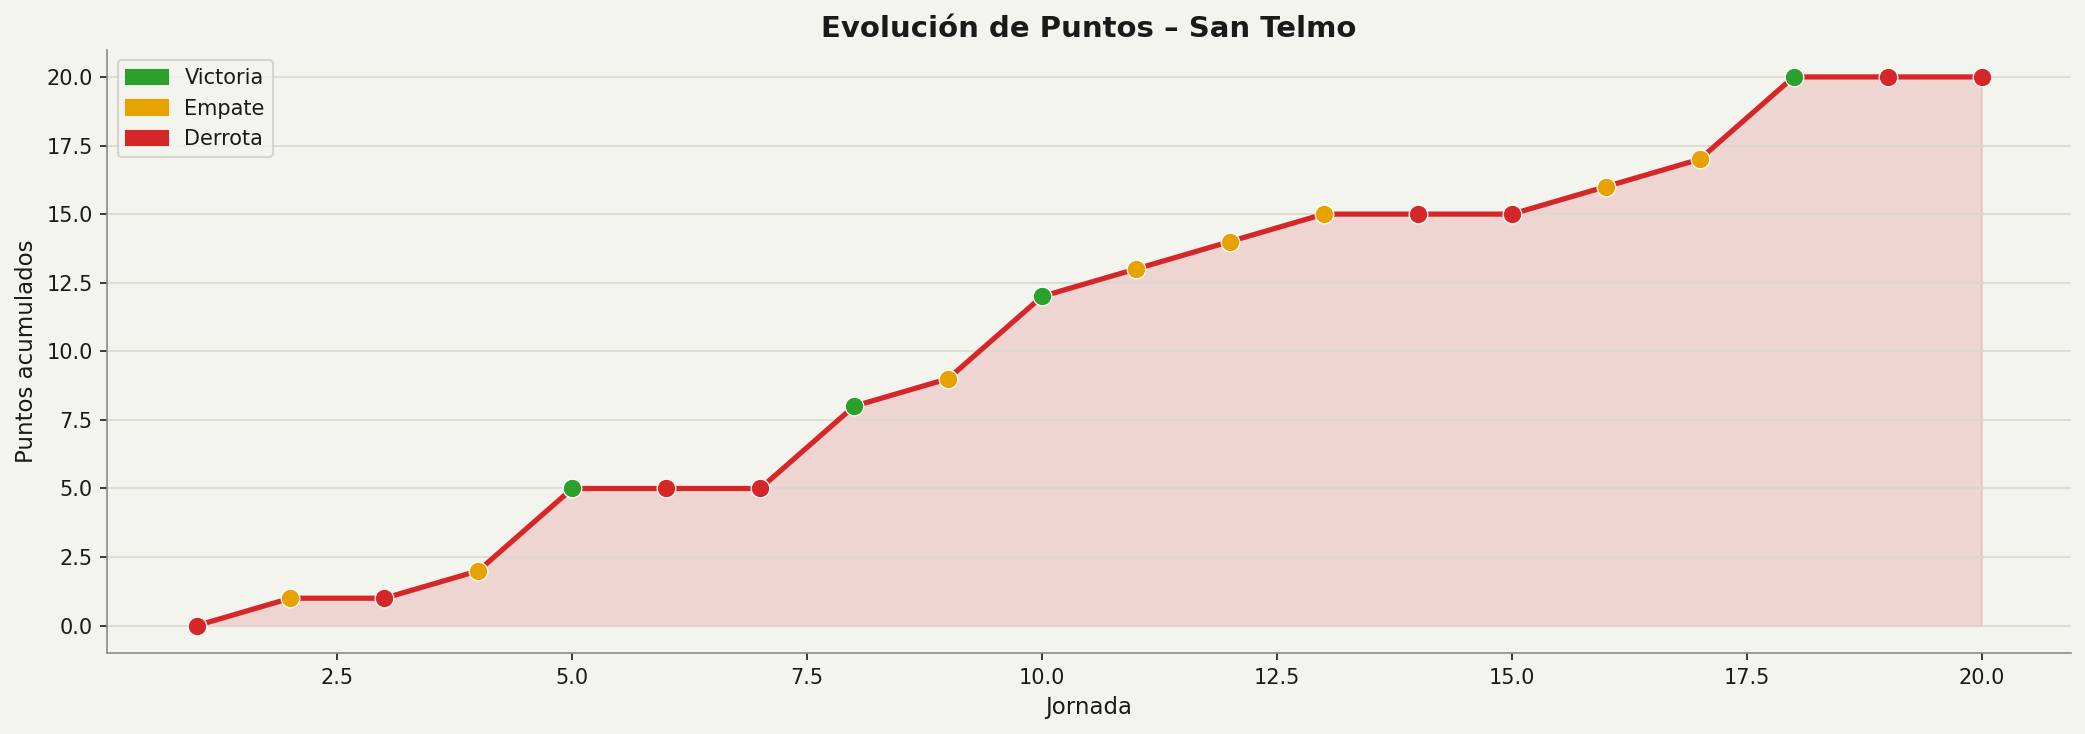
\includegraphics[width=0.9\textwidth]{puntos_acumulados.png}}
  \caption{Puntos acumulados de San Telmo a lo largo de la temporada.}
\end{figure}

\begin{figure}[htbp]
  \centering
  \fbox{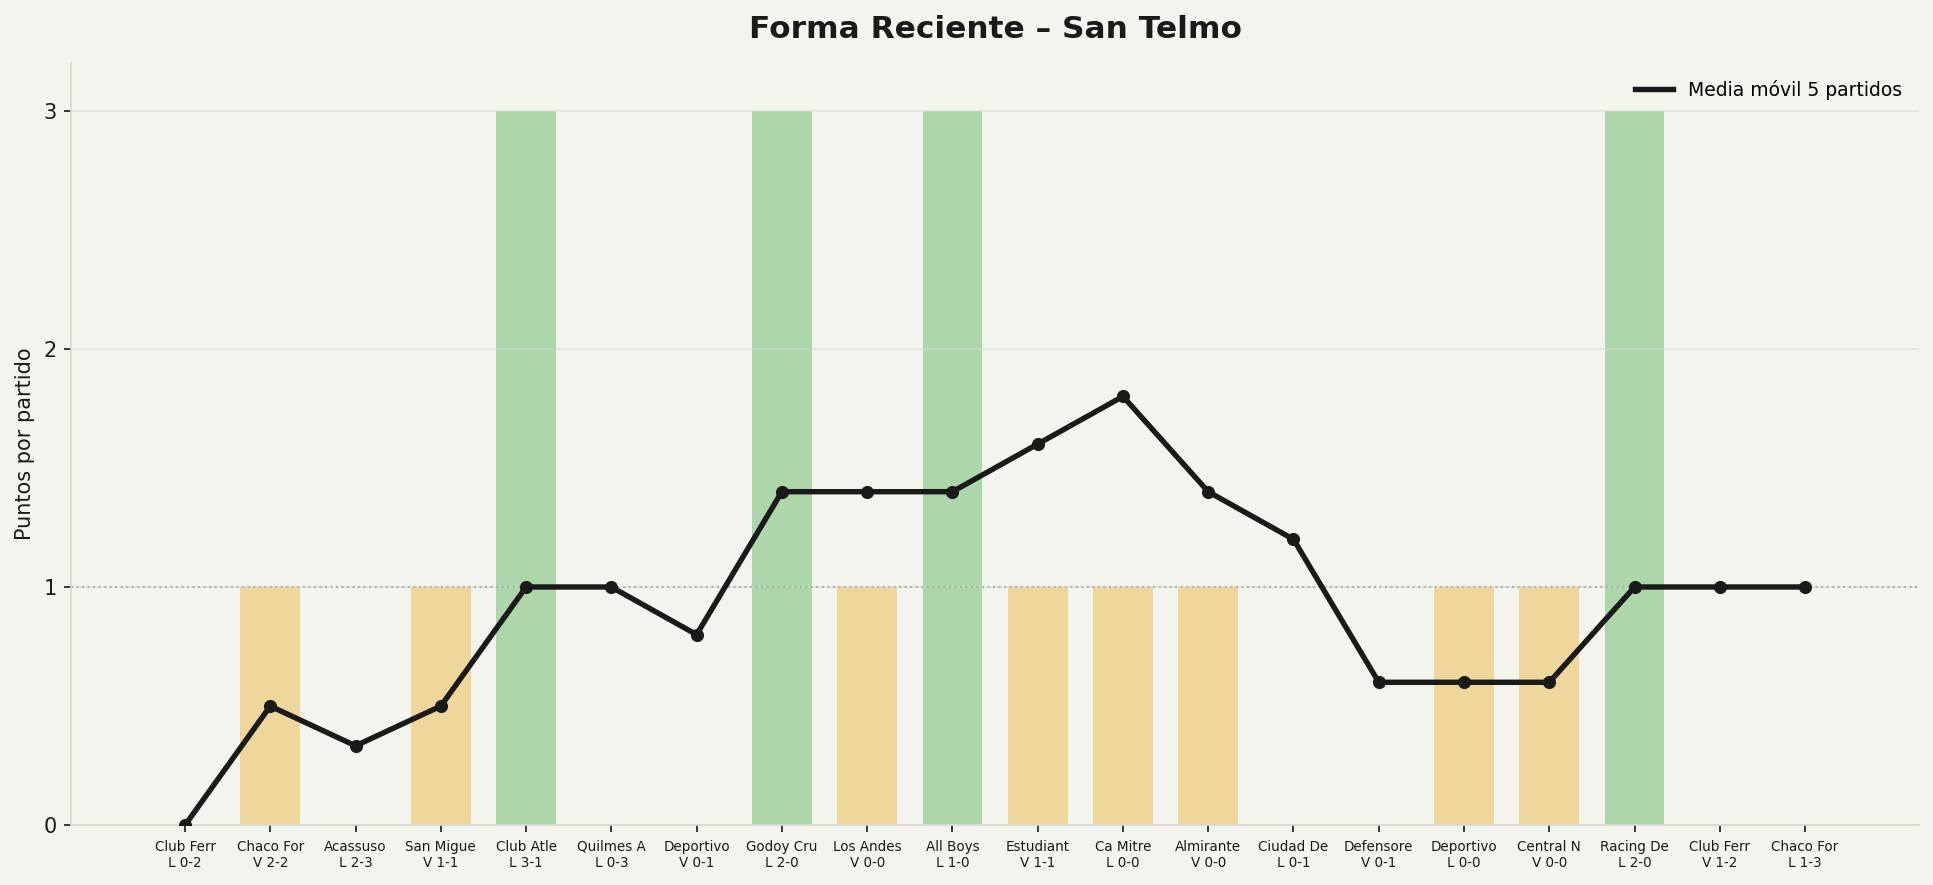
\includegraphics[width=0.9\textwidth]{forma_reciente.png}}
  \caption{Forma reciente (media móvil de 5 partidos): rachas por encima y por debajo del promedio.}
\end{figure}

\slot{lectura general del momento del equipo}

\section*{2. Ataque}
Volumen y calidad de las situaciones de gol generadas: de dónde patea, qué tan variado es su ataque y por qué vías genera peligro.

\begin{figure}[htbp]
  \centering
  \fbox{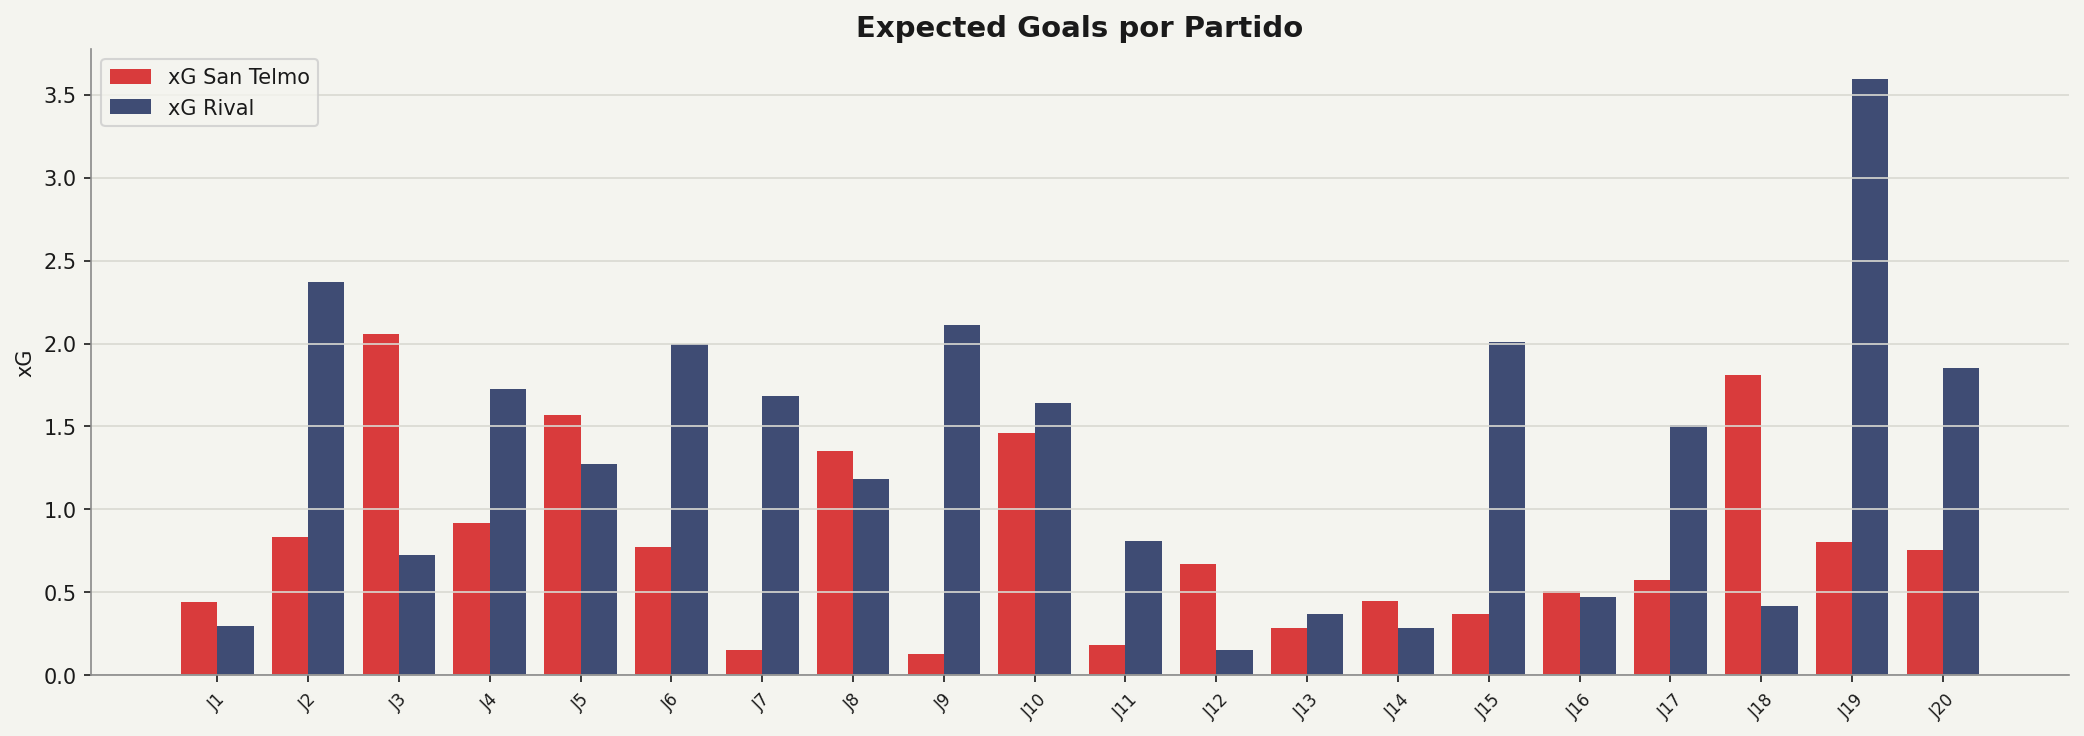
\includegraphics[width=0.9\textwidth]{xg_temporada.png}}
  \caption{Goles vs. xG a lo largo de la temporada: eficacia en la definición.}
\end{figure}

\begin{figure}[htbp]
  \centering
  \fbox{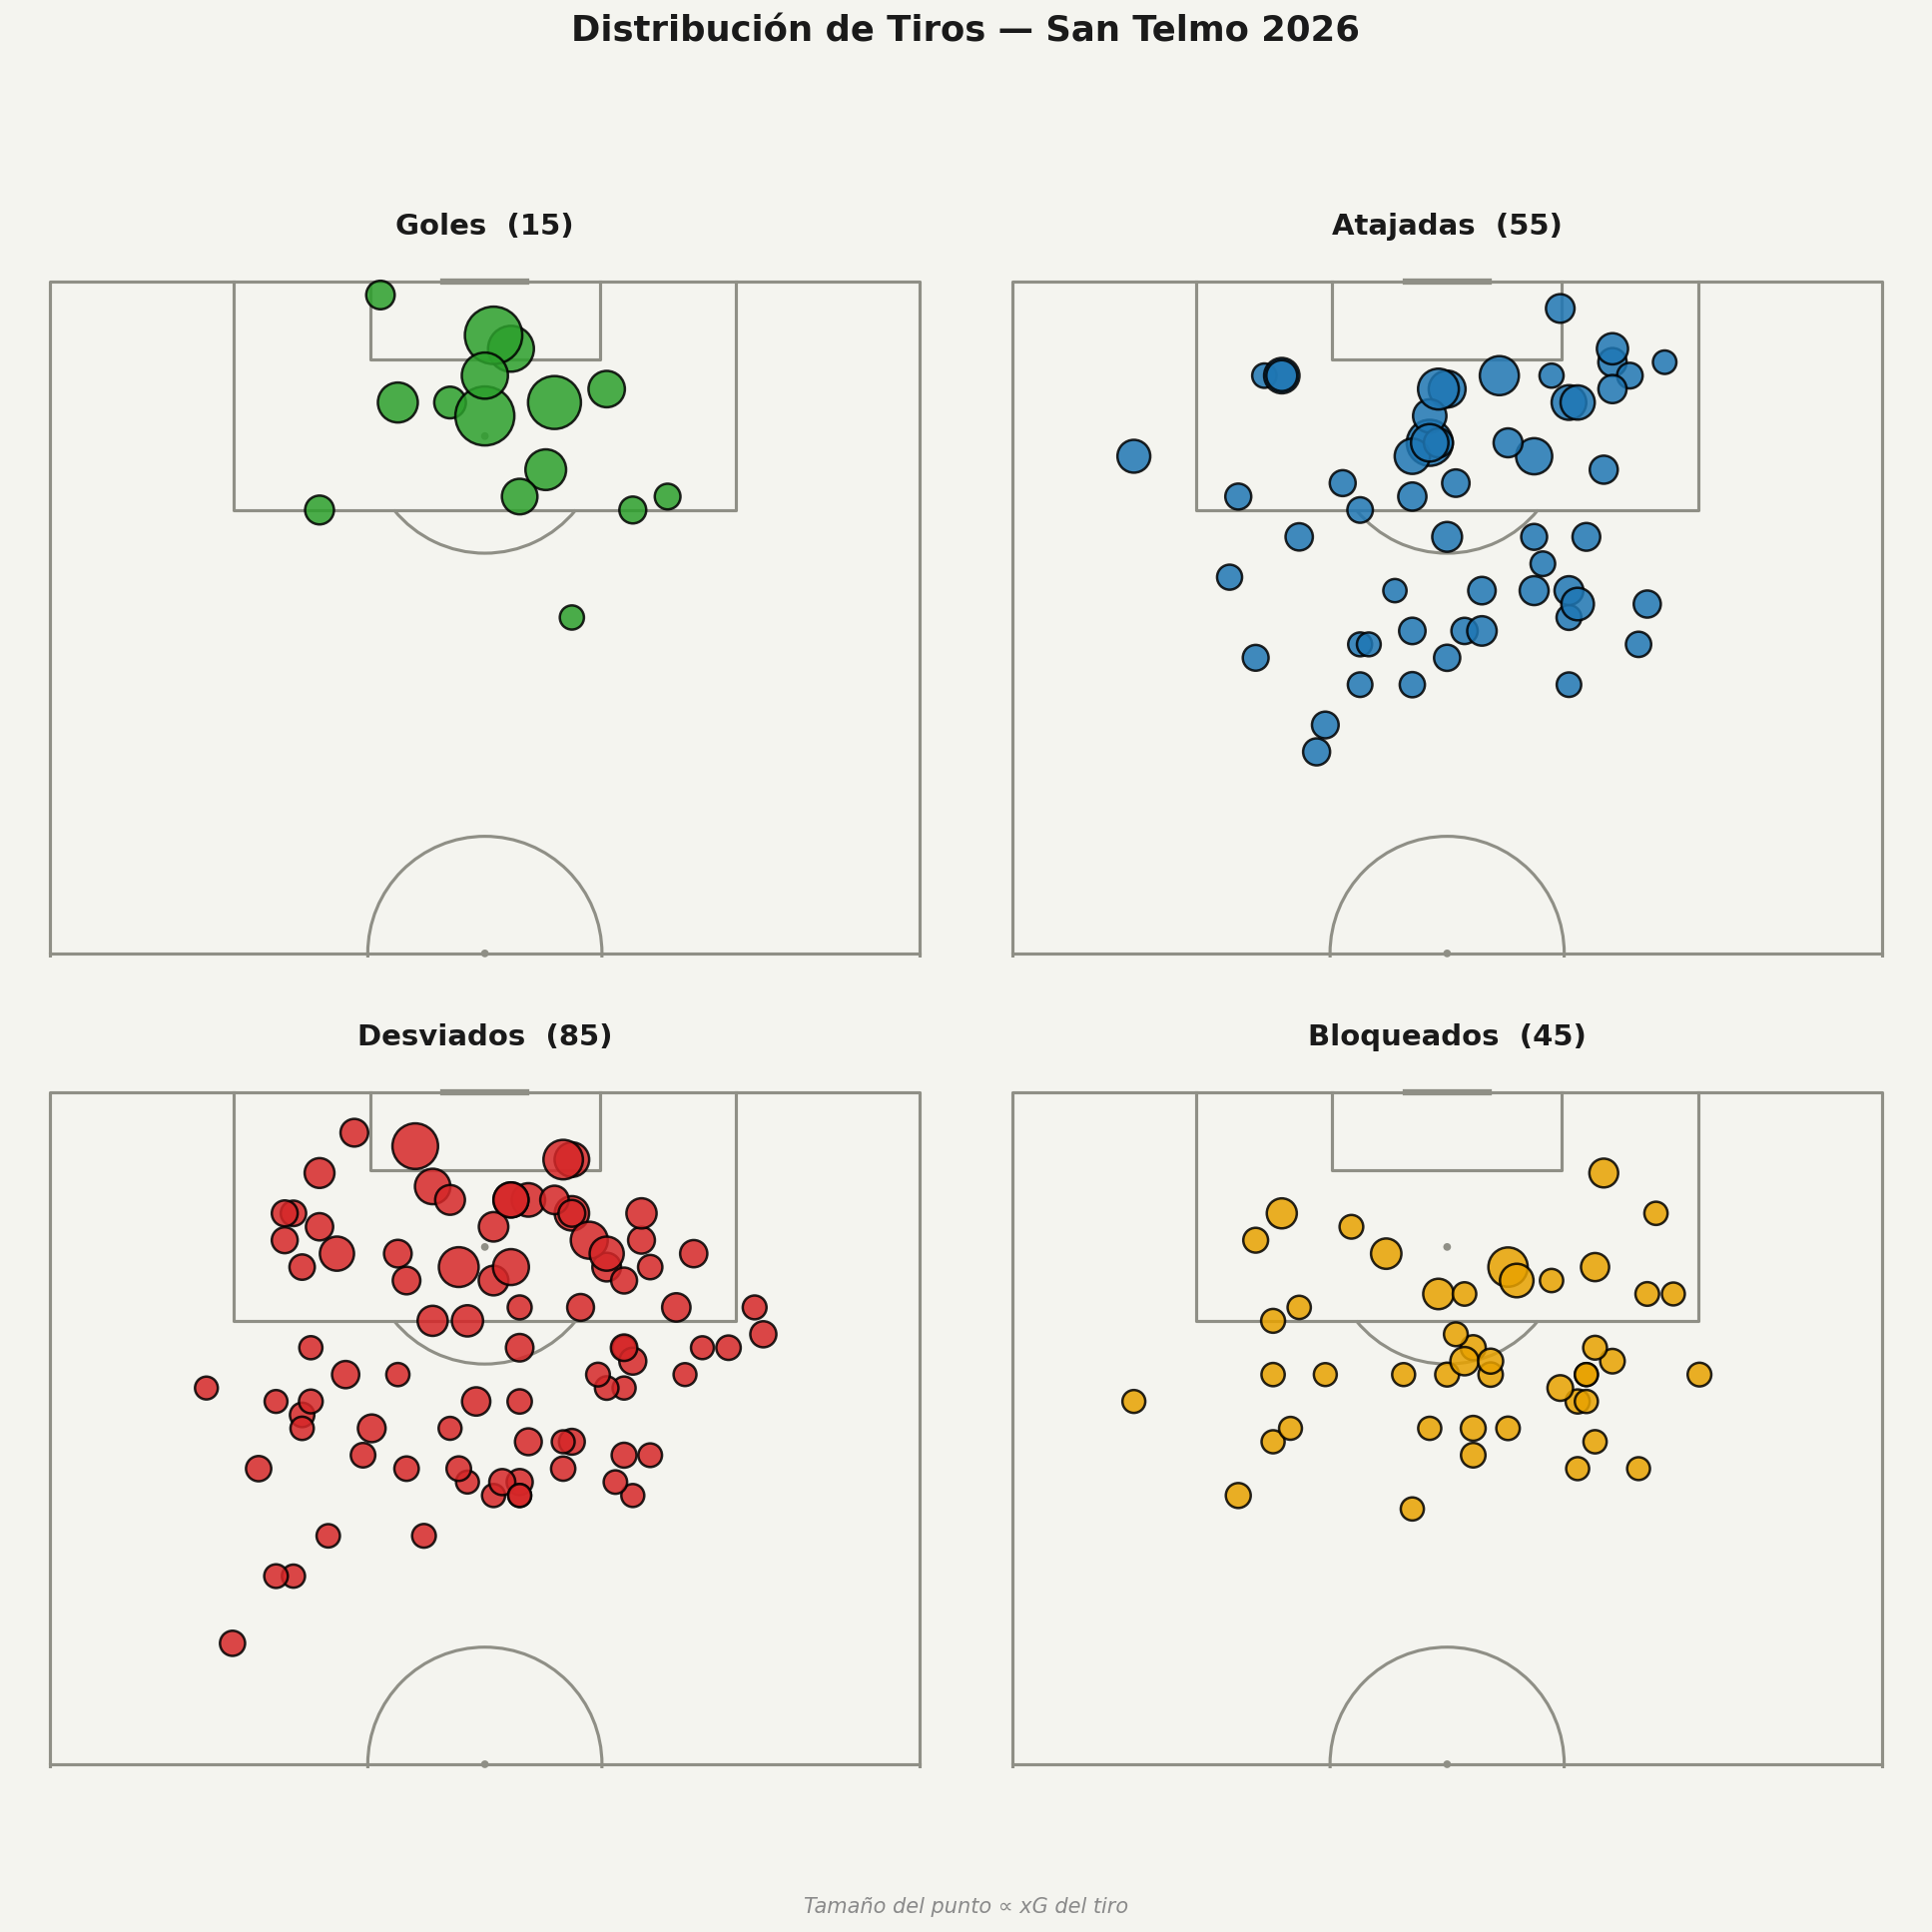
\includegraphics[width=0.98\textwidth]{shotmap_temporada.png}}
  \caption{Mapa de tiros de la temporada (gol / atajado / desviado / bloqueado); tamaño del punto según xG.}
\end{figure}

\begin{figure}[htbp]
  \centering
  \fbox{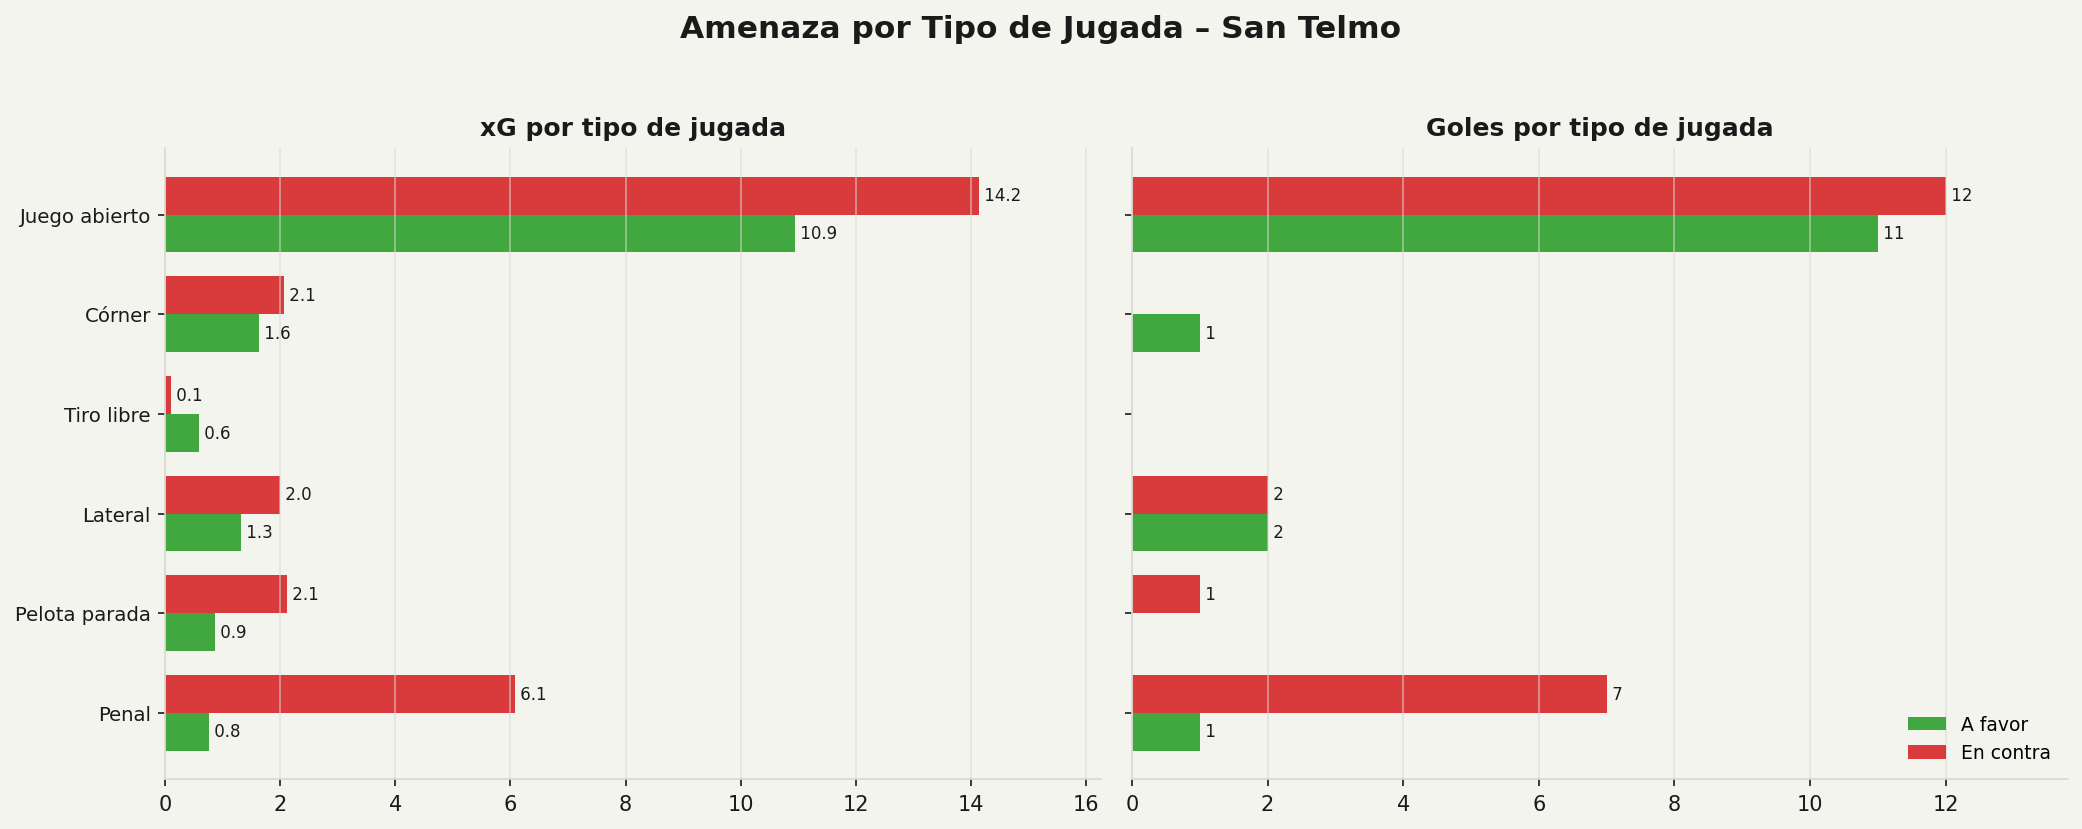
\includegraphics[width=0.98\textwidth]{amenaza_por_jugada.png}}
  \caption{Amenaza por tipo de jugada: goles y xG a favor y en contra según la situación (juego abierto, pelota parada, etc.).}
\end{figure}

\begin{figure}[htbp]
  \centering
  \fbox{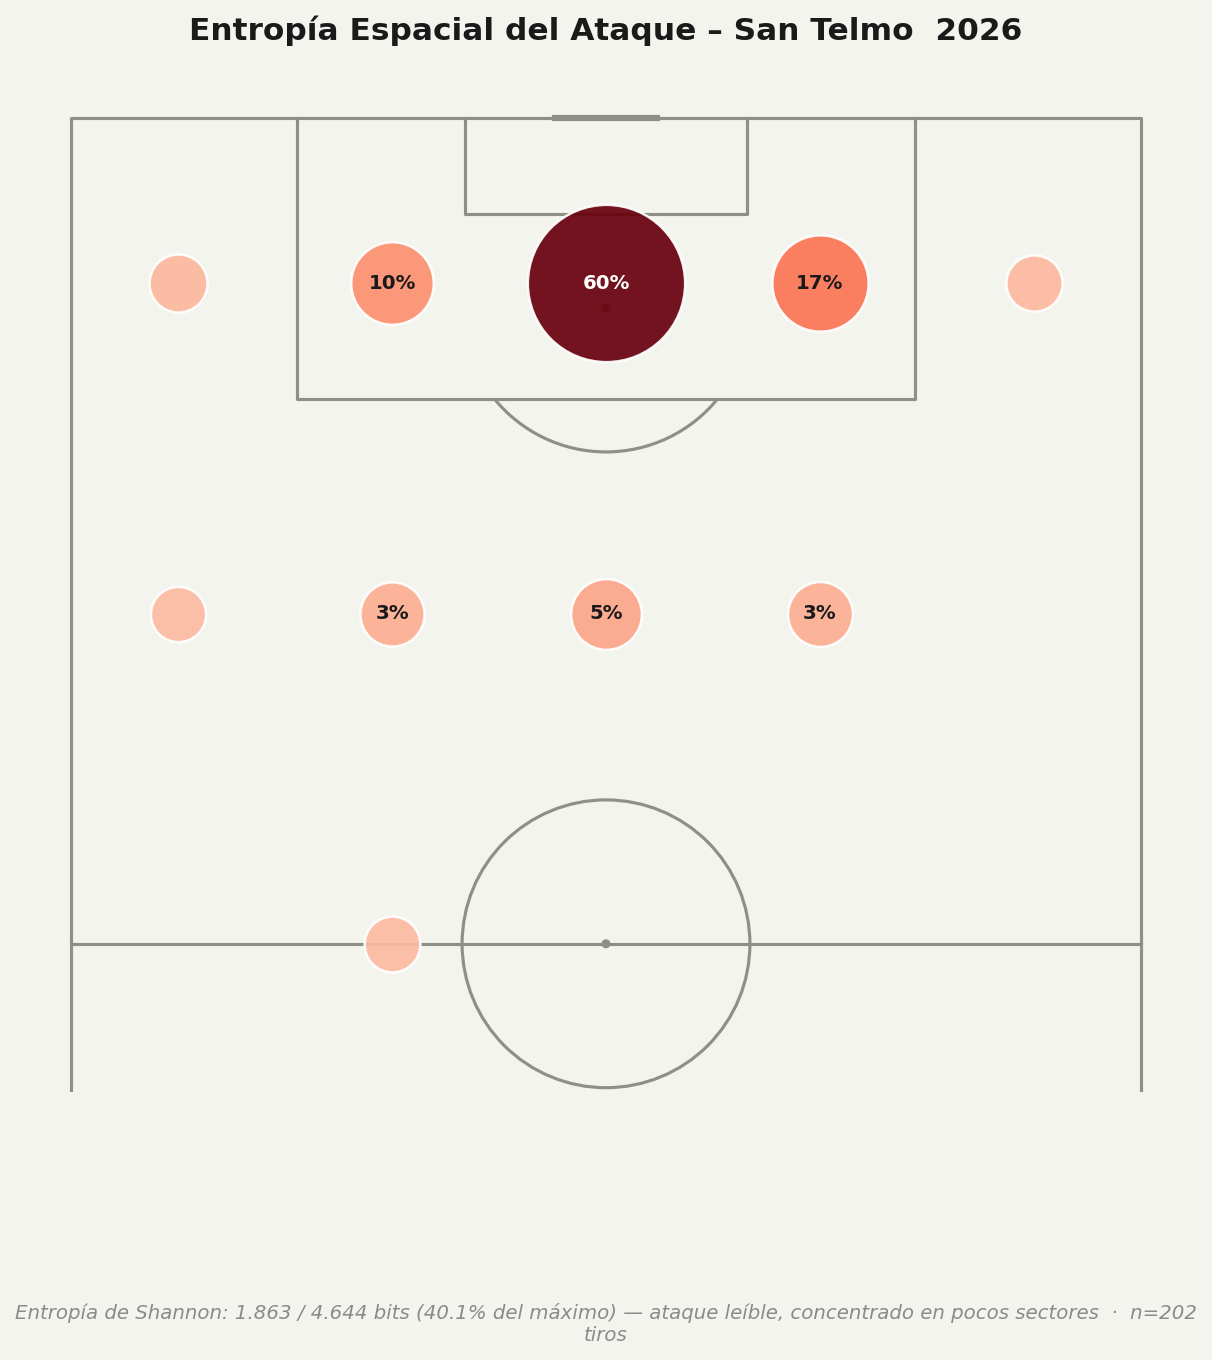
\includegraphics[width=0.6\textwidth]{entropia_tiros.png}}
  \caption{Entropía del mapa de tiros: qué tan predecible o variado es el origen del peligro.}
\end{figure}

\begin{figure}[htbp]
  \centering
  \fbox{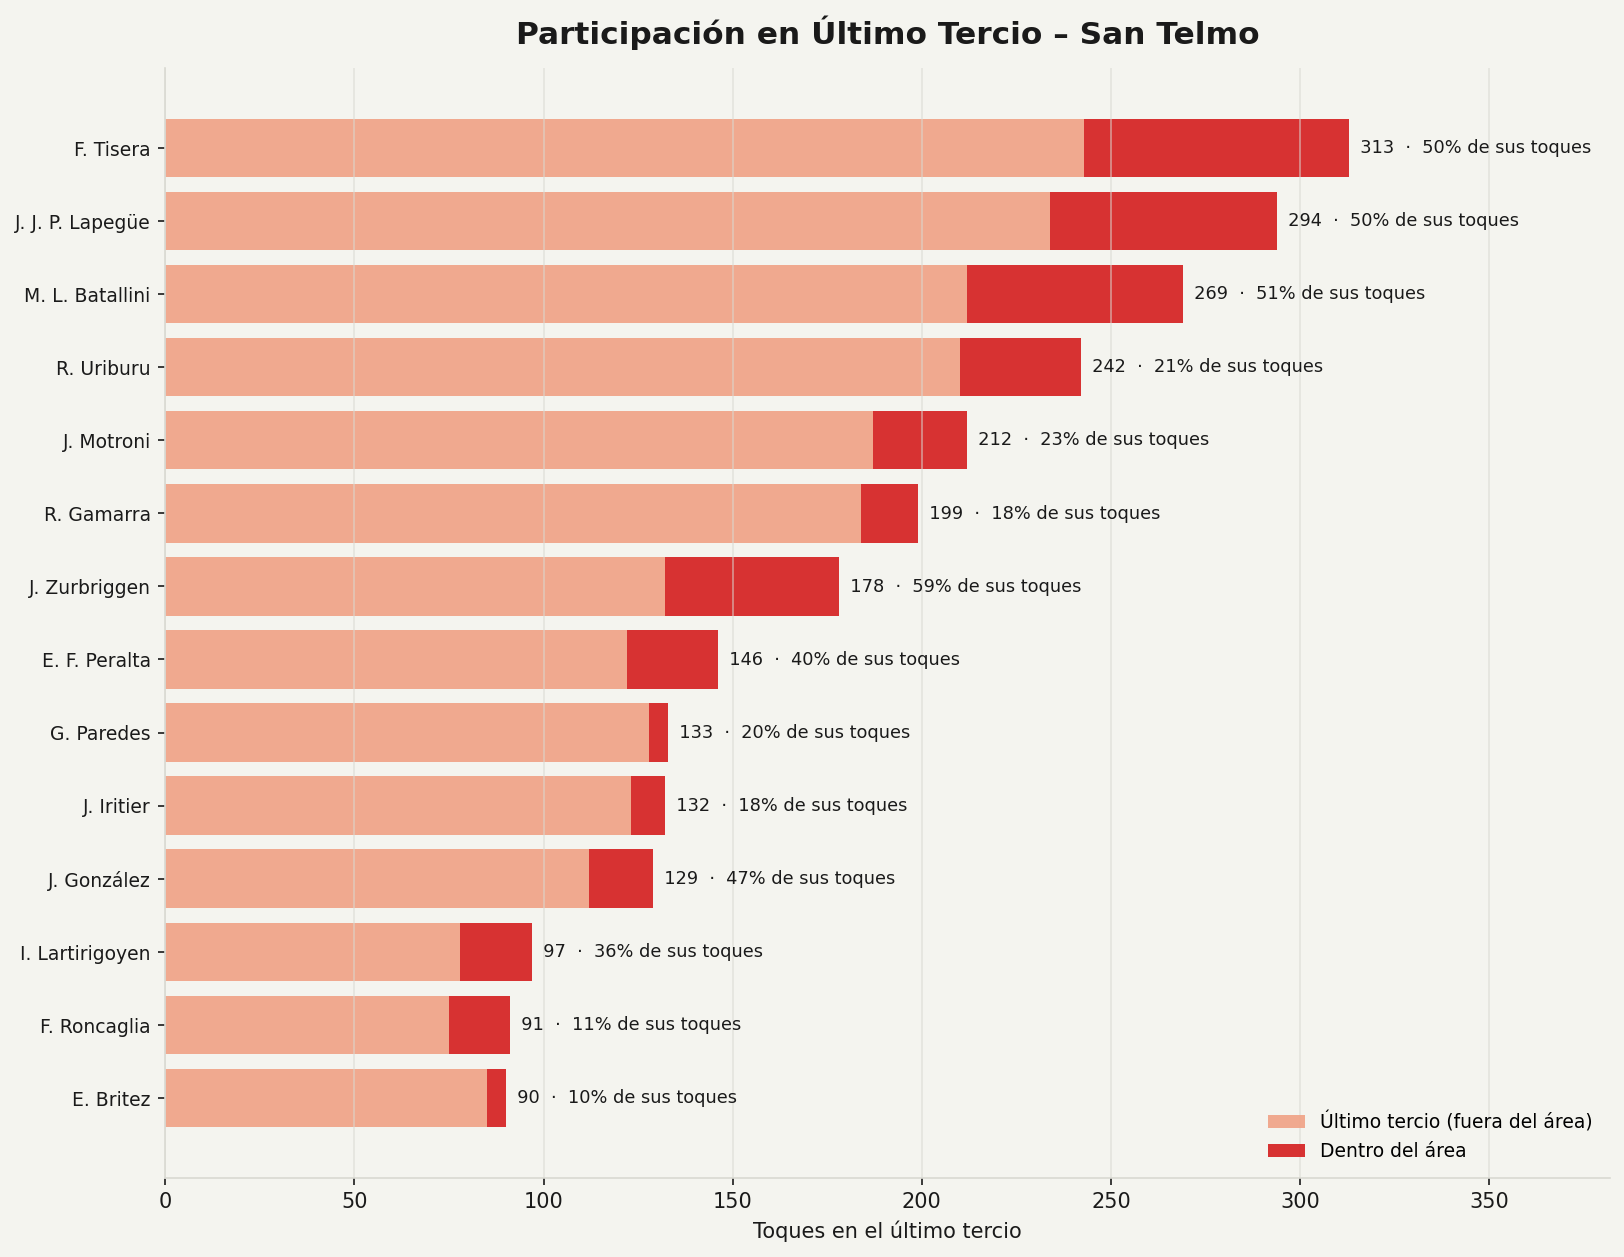
\includegraphics[width=0.9\textwidth]{toques_ultimo_tercio.png}}
  \caption{Toques en el último tercio / área rival por jugador: participación ofensiva real.}
\end{figure}

\slot{fortalezas y vías de peligro del ataque}

\section*{3. Defensa y Gestión del Partido}
\begin{figure}[htbp]
  \centering
  \fbox{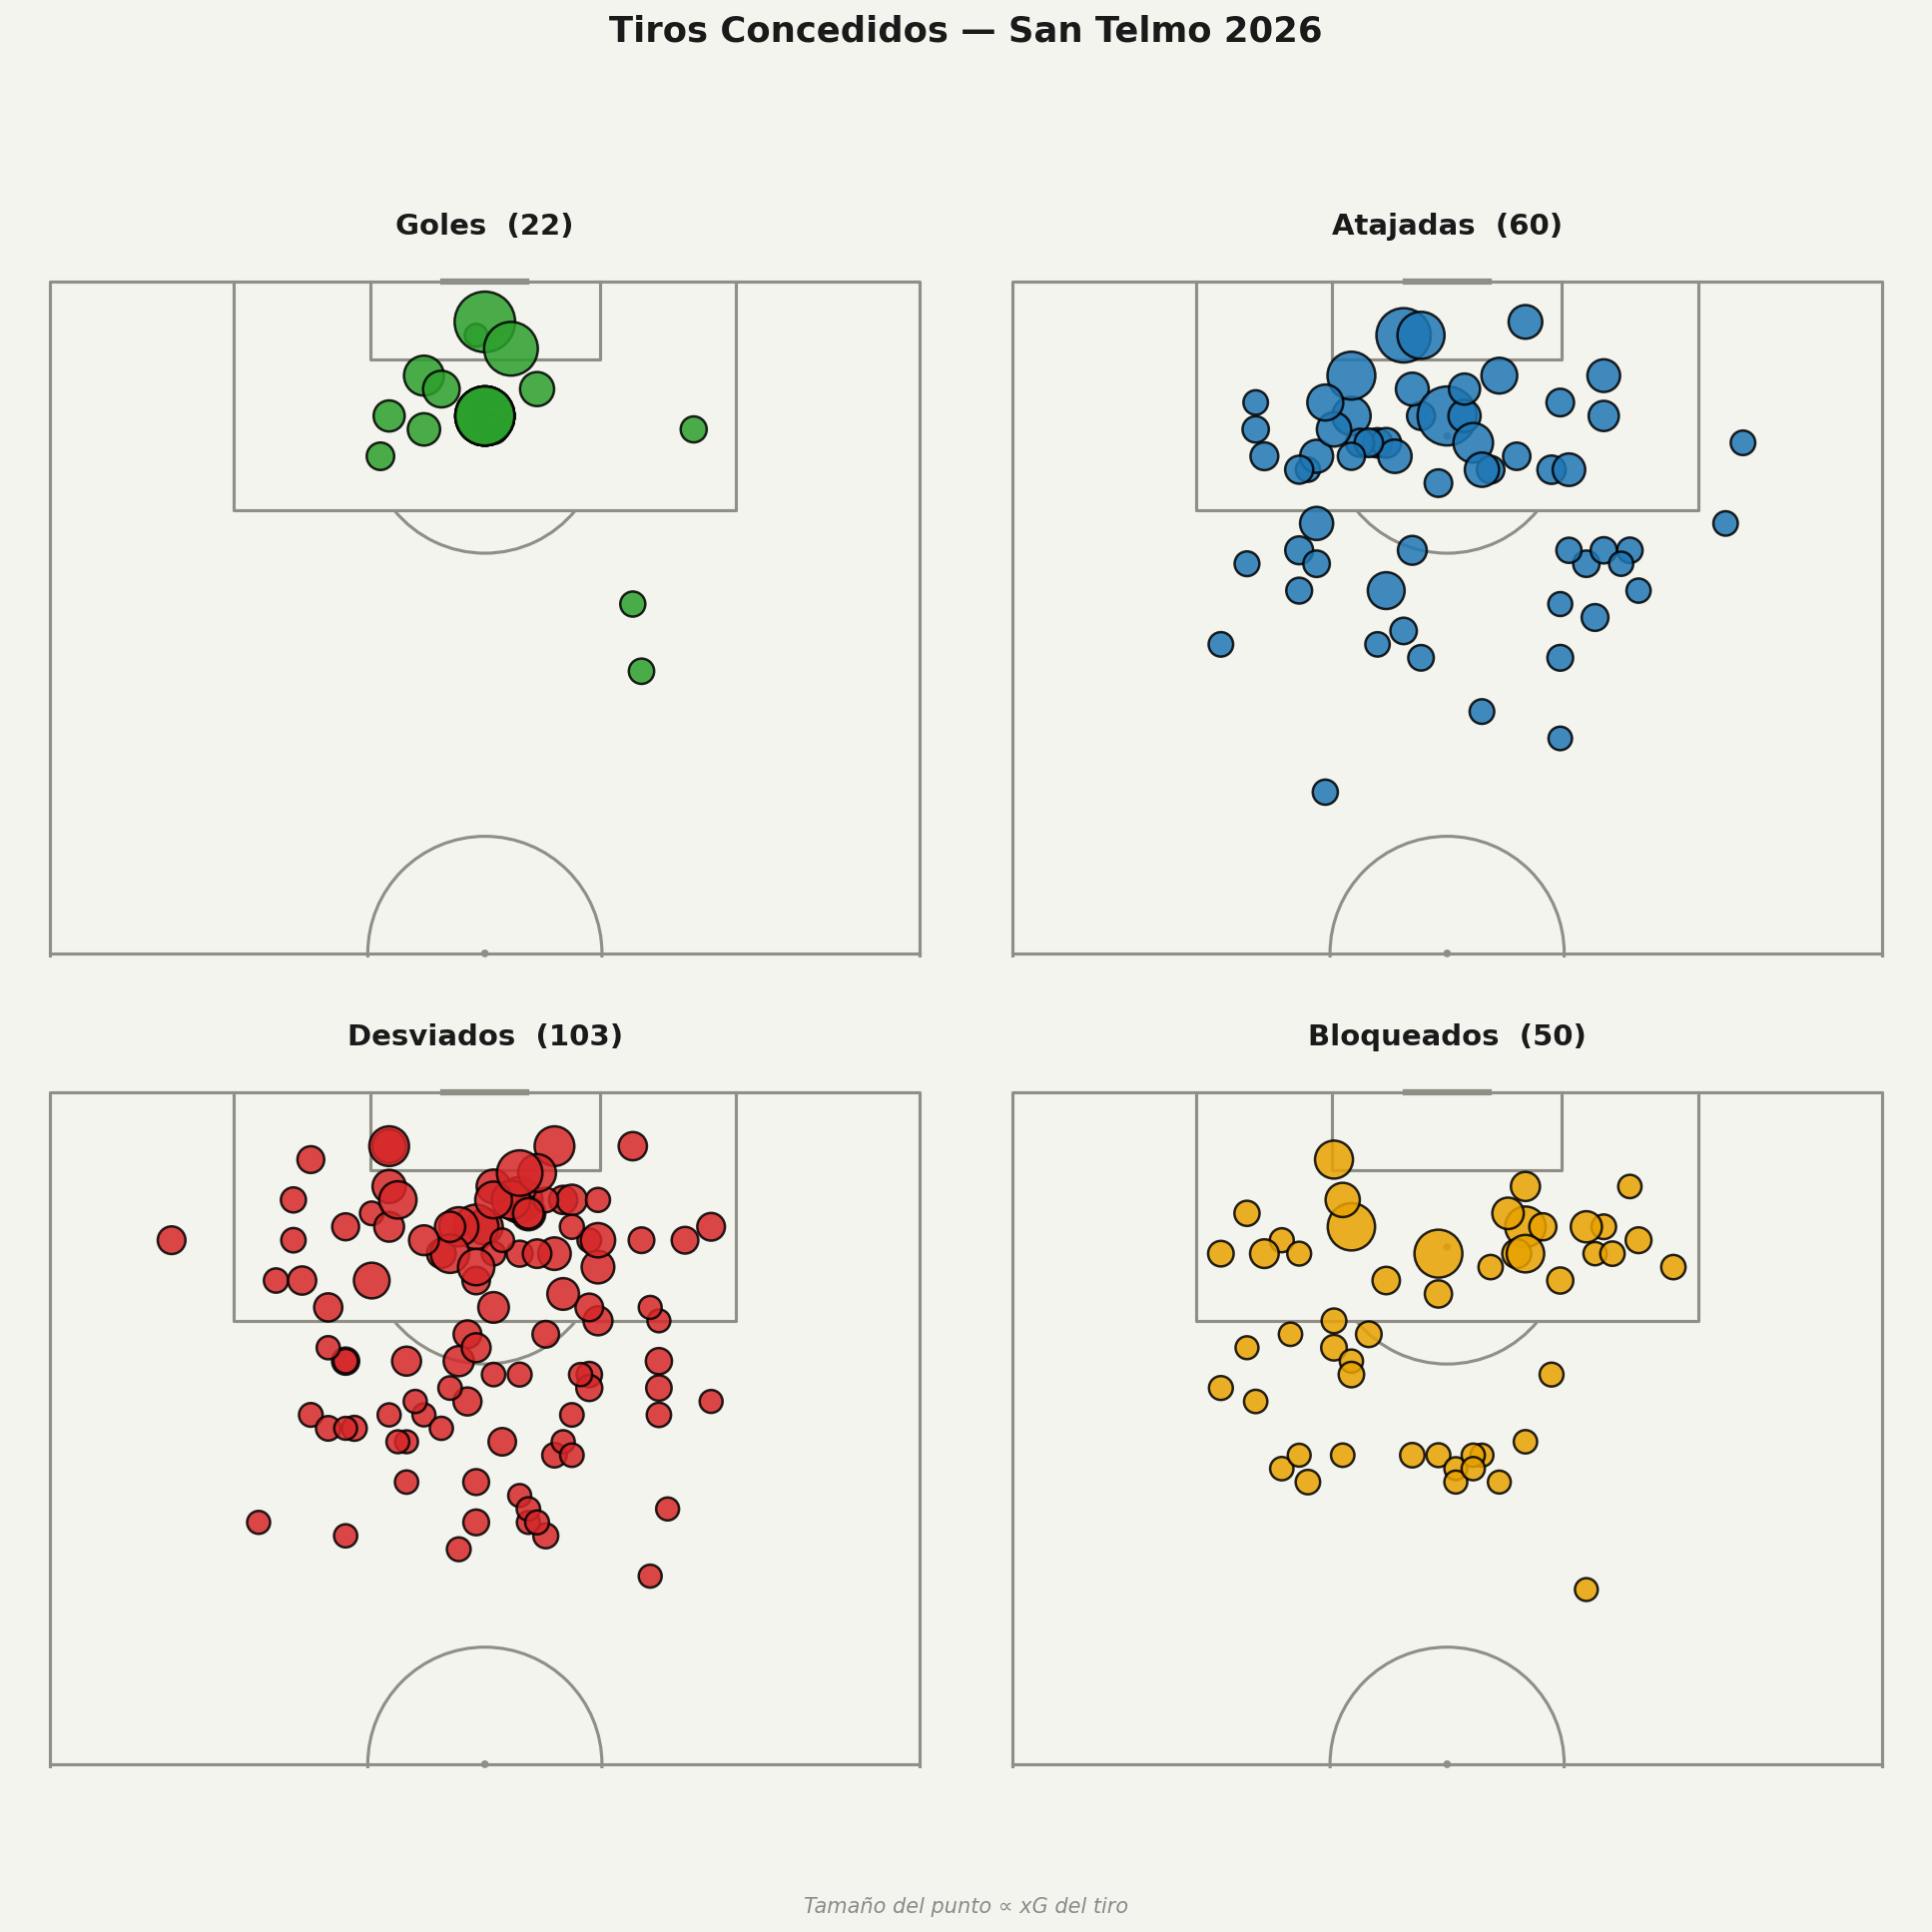
\includegraphics[width=0.98\textwidth]{tiros_concedidos_temporada.png}}
  \caption{Mapa de tiros concedidos: dónde le generan peligro al equipo durante el año.}
\end{figure}

\begin{figure}[htbp]
  \centering
  \fbox{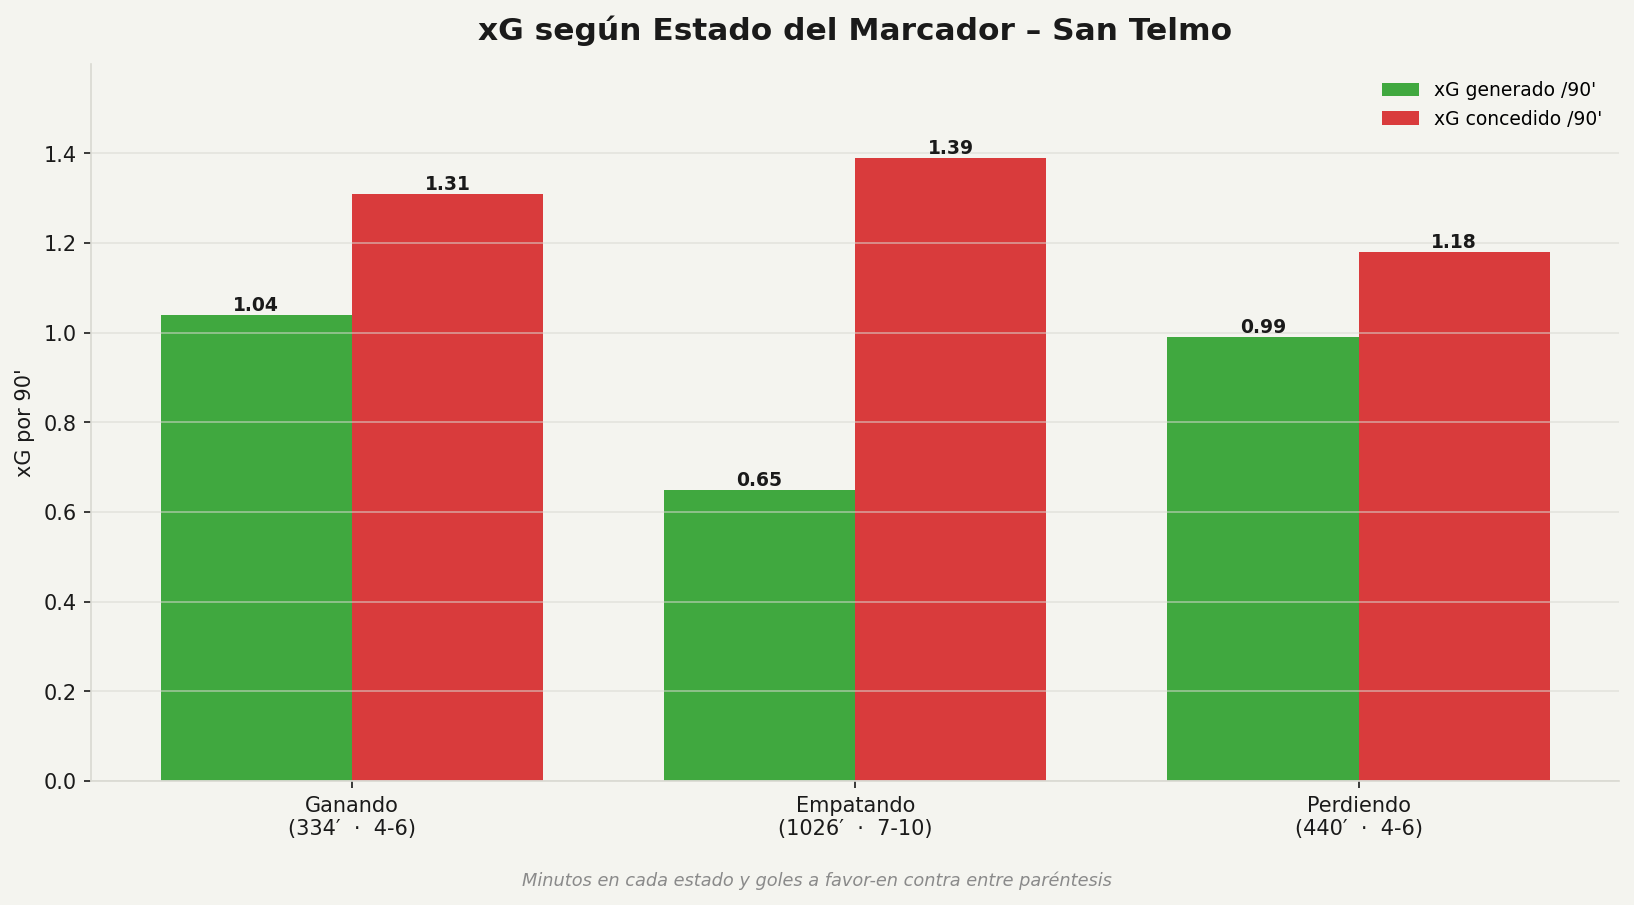
\includegraphics[width=0.9\textwidth]{xg_por_estado_marcador.png}}
  \caption{xG generado y concedido según el estado del marcador: cómo gestiona ir ganando, empatando o perdiendo.}
\end{figure}

\begin{figure}[htbp]
  \centering
  \fbox{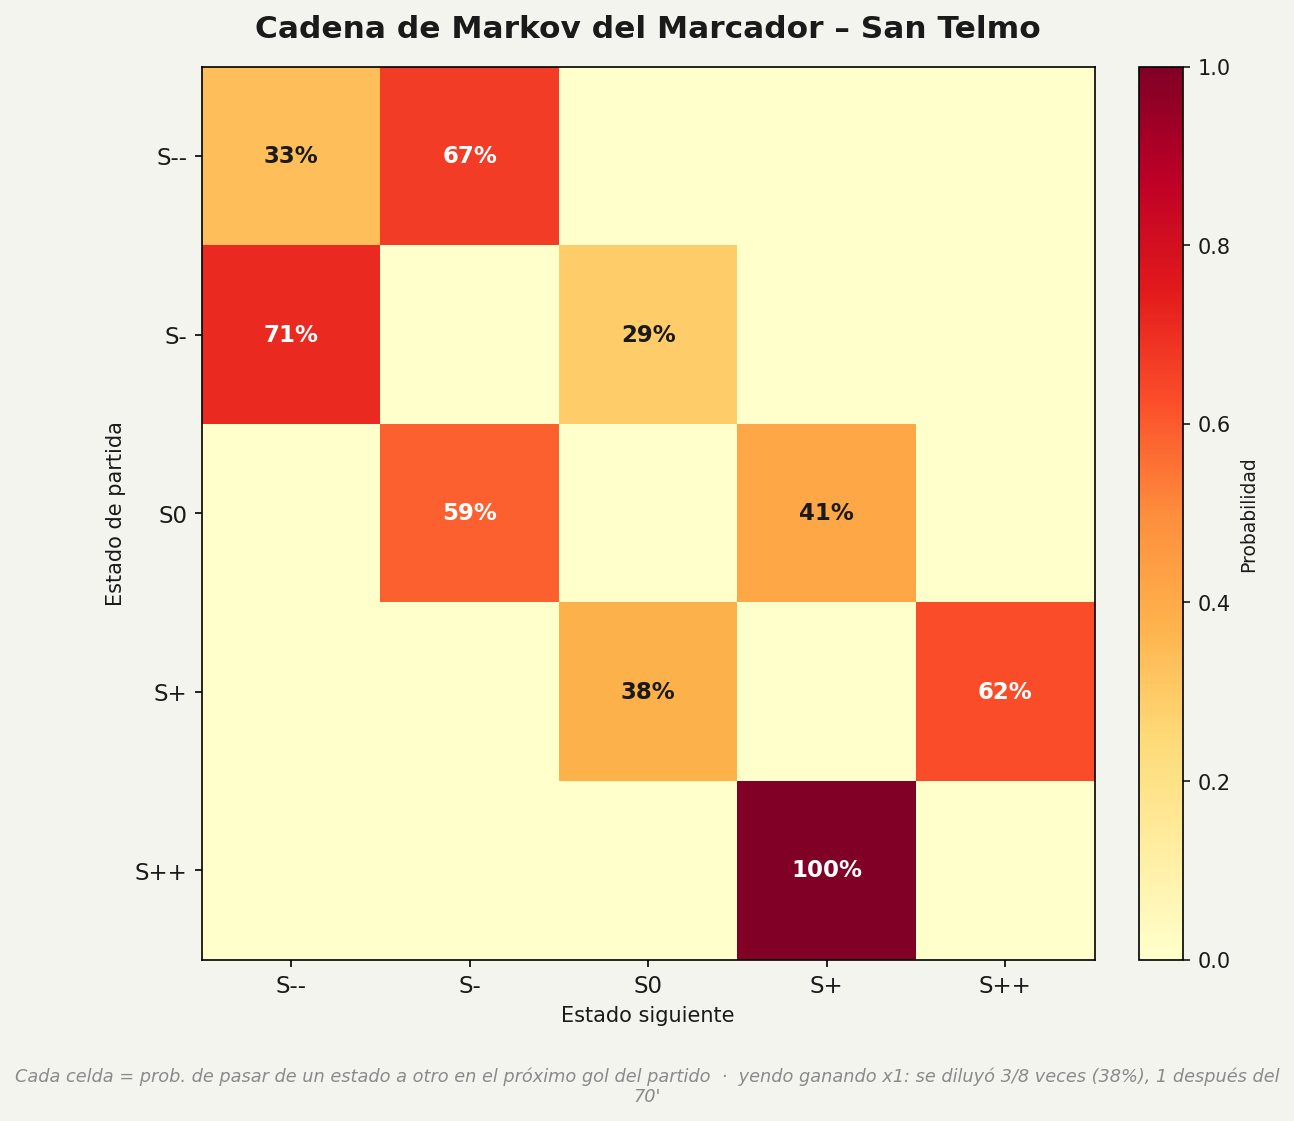
\includegraphics[width=0.6\textwidth]{markov_marcador.png}}
  \caption{Cadena de Markov del marcador: probabilidad de mover el resultado gol a gol (madurez para sostener o revertir).}
\end{figure}

\begin{figure}[htbp]
  \centering
  \fbox{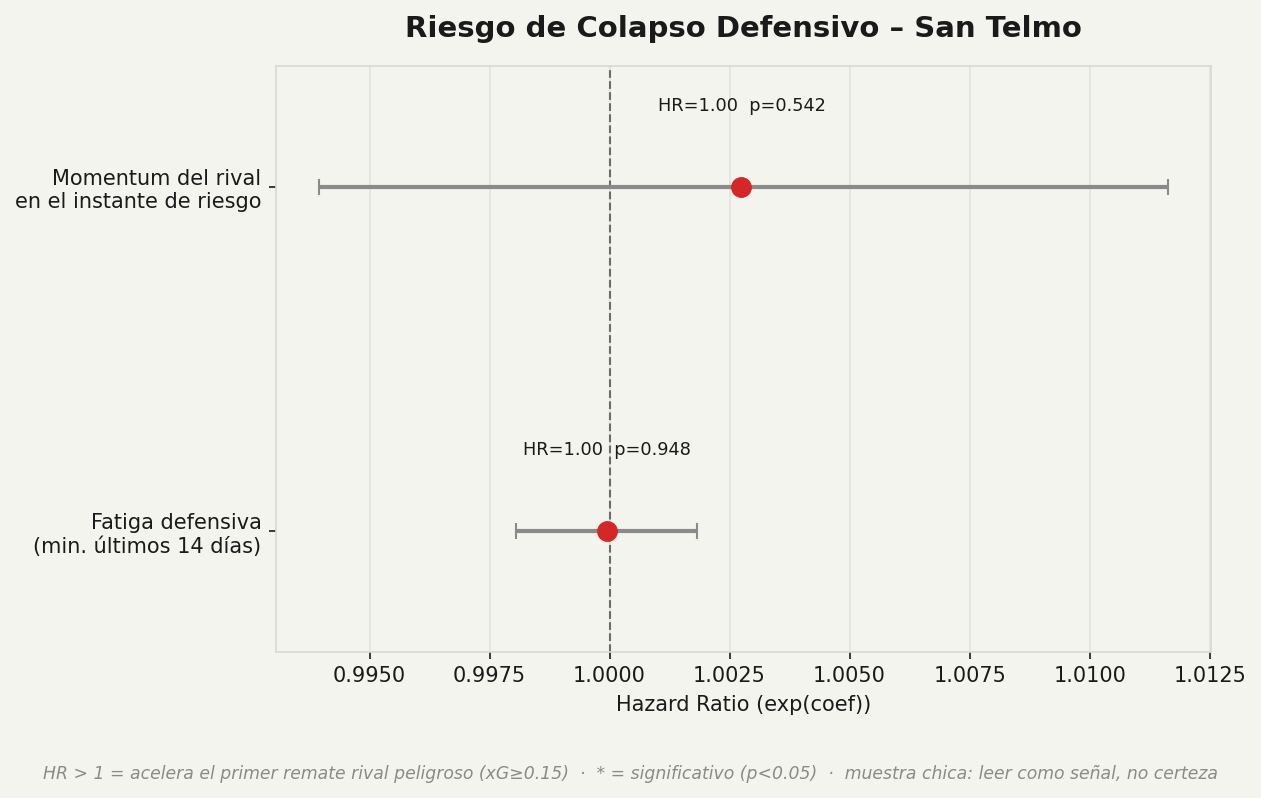
\includegraphics[width=0.85\textwidth]{riesgo_defensivo_cox.png}}
  \caption{Modelo de riesgo defensivo (Cox): factores asociados a recibir el primer remate peligroso. Señal direccional.}
\end{figure}

\slot{solidez defensiva y momentos de riesgo}

\section*{4. Jugadores y Plantel}
\subsection*{Goleadores}
\begin{table}[h!]\centering\begin{tabular}{lccc}\toprule
\textbf{Jugador} & \textbf{Goles} & \textbf{xG} & \textbf{PJ} \\\midrule
M. L. Batallini & 2 & 2.08 & 18 \\
F. Tisera & 2 & 1.52 & 17 \\
J. Motroni & 2 & 0.53 & 19 \\
J. González & 2 & 0.46 & 10 \\
F. Roncaglia & 1 & 0.43 & 13 \\
\bottomrule\end{tabular}\end{table}

\subsection*{Mejores promedios (mín. 600')}
\begin{table}[h!]\centering\begin{tabular}{lccc}\toprule
\textbf{Jugador} & \textbf{Rating} & \textbf{Min} & \textbf{PJ} \\\midrule
J. Enrico & 7.22 & 1800 & 20 \\
R. Gamarra & 7.11 & 1303 & 20 \\
L. Pollacchi & 6.93 & 1628 & 20 \\
F. Roncaglia & 6.86 & 989 & 13 \\
J. Motroni & 6.84 & 1097 & 19 \\
\bottomrule\end{tabular}\end{table}

\begin{figure}[htbp]
  \centering
  \fbox{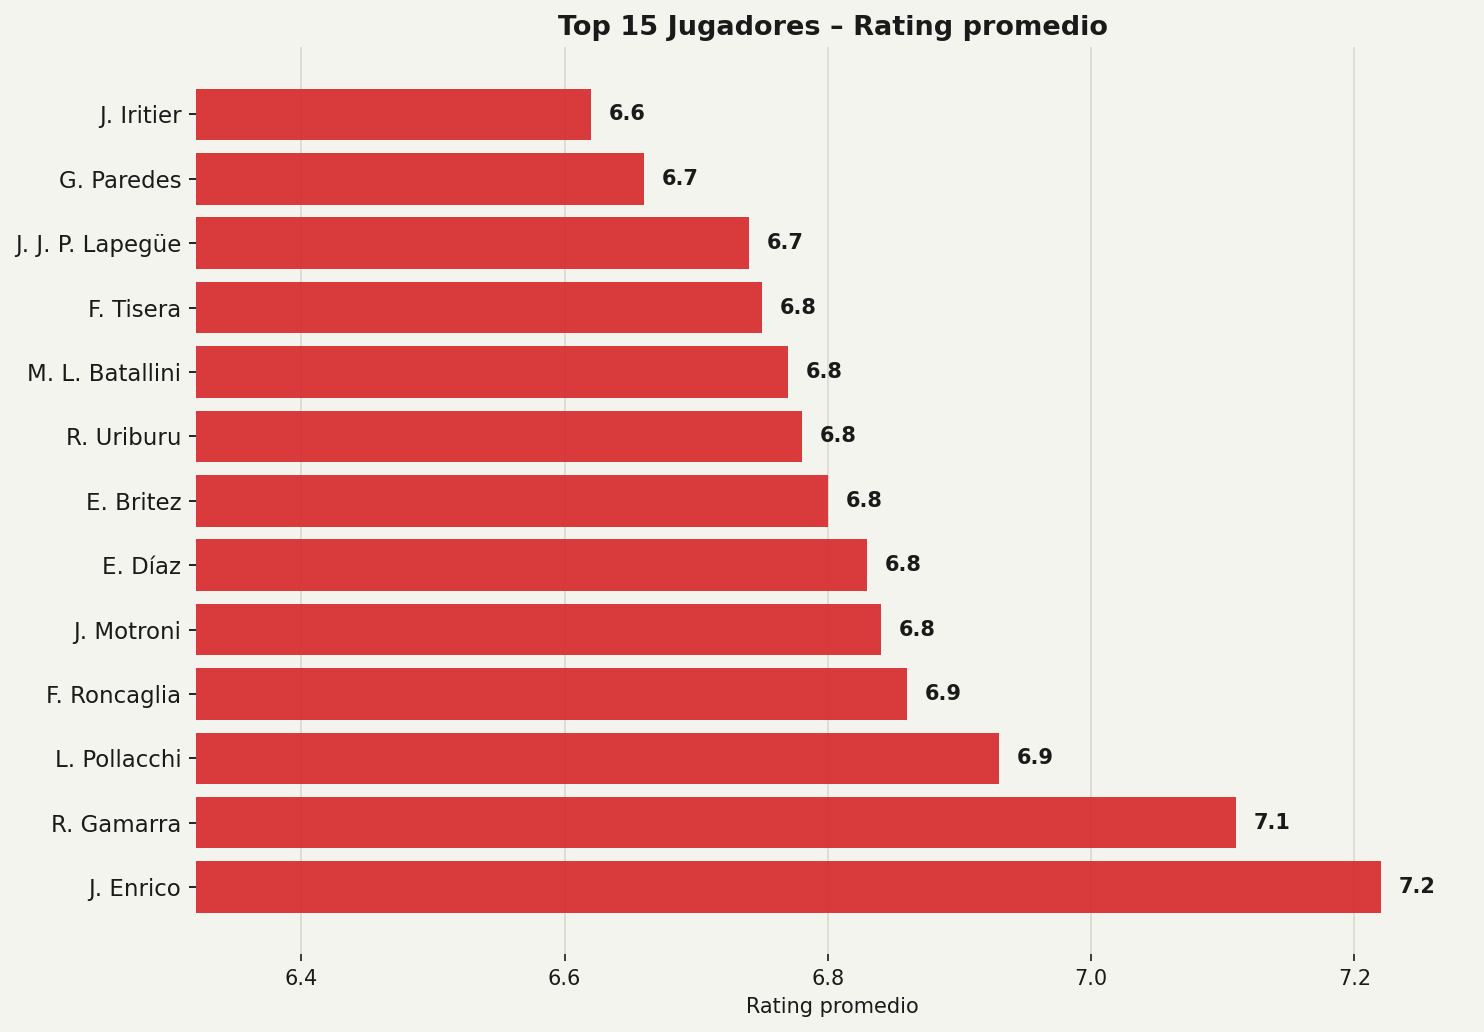
\includegraphics[width=0.9\textwidth]{top_rating.png}}
  \caption{Jugadores mejor puntuados de la temporada (mínimo 600 minutos).}
\end{figure}

\begin{figure}[htbp]
  \centering
  \fbox{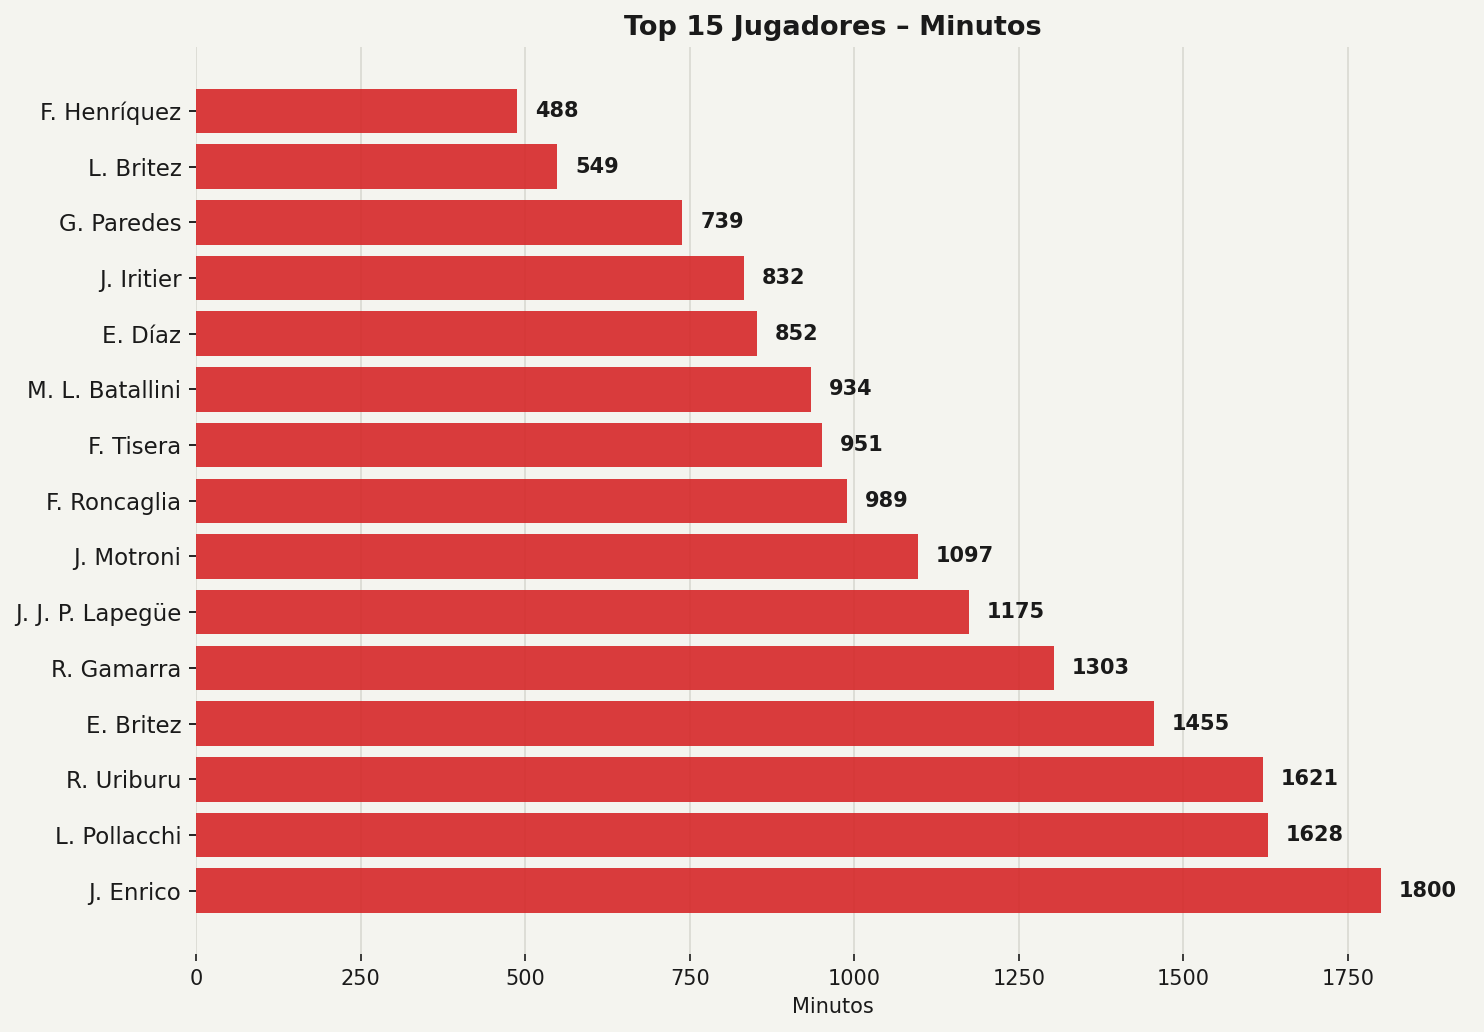
\includegraphics[width=0.9\textwidth]{top_minutos.png}}
  \caption{Jugadores más utilizados por minutos.}
\end{figure}

\begin{figure}[htbp]
  \centering
  \fbox{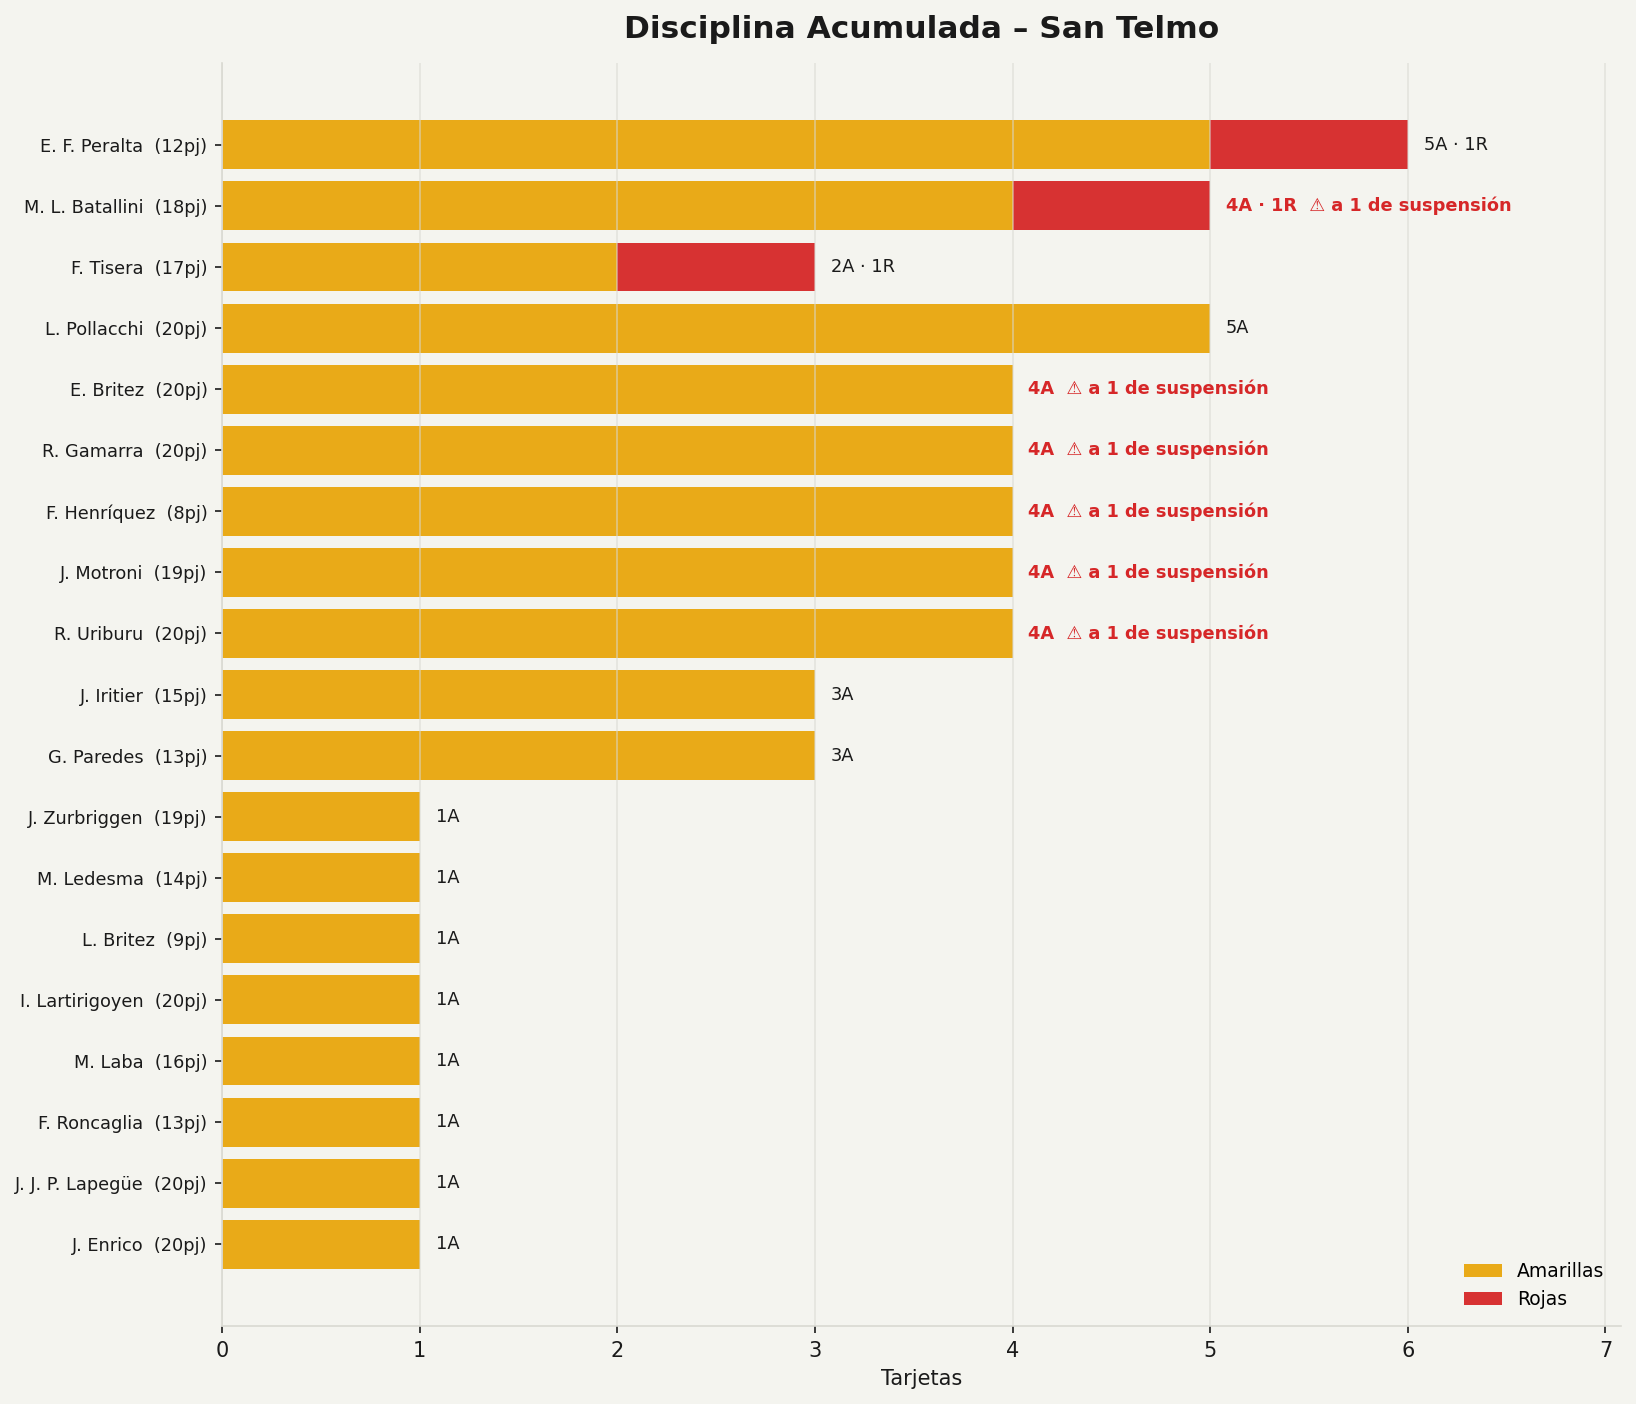
\includegraphics[width=0.9\textwidth]{disciplina.png}}
  \caption{Disciplina: amarillas y rojas por jugador; marca a los que están al borde de la suspensión.}
\end{figure}

\begin{figure}[htbp]
  \centering
  \fbox{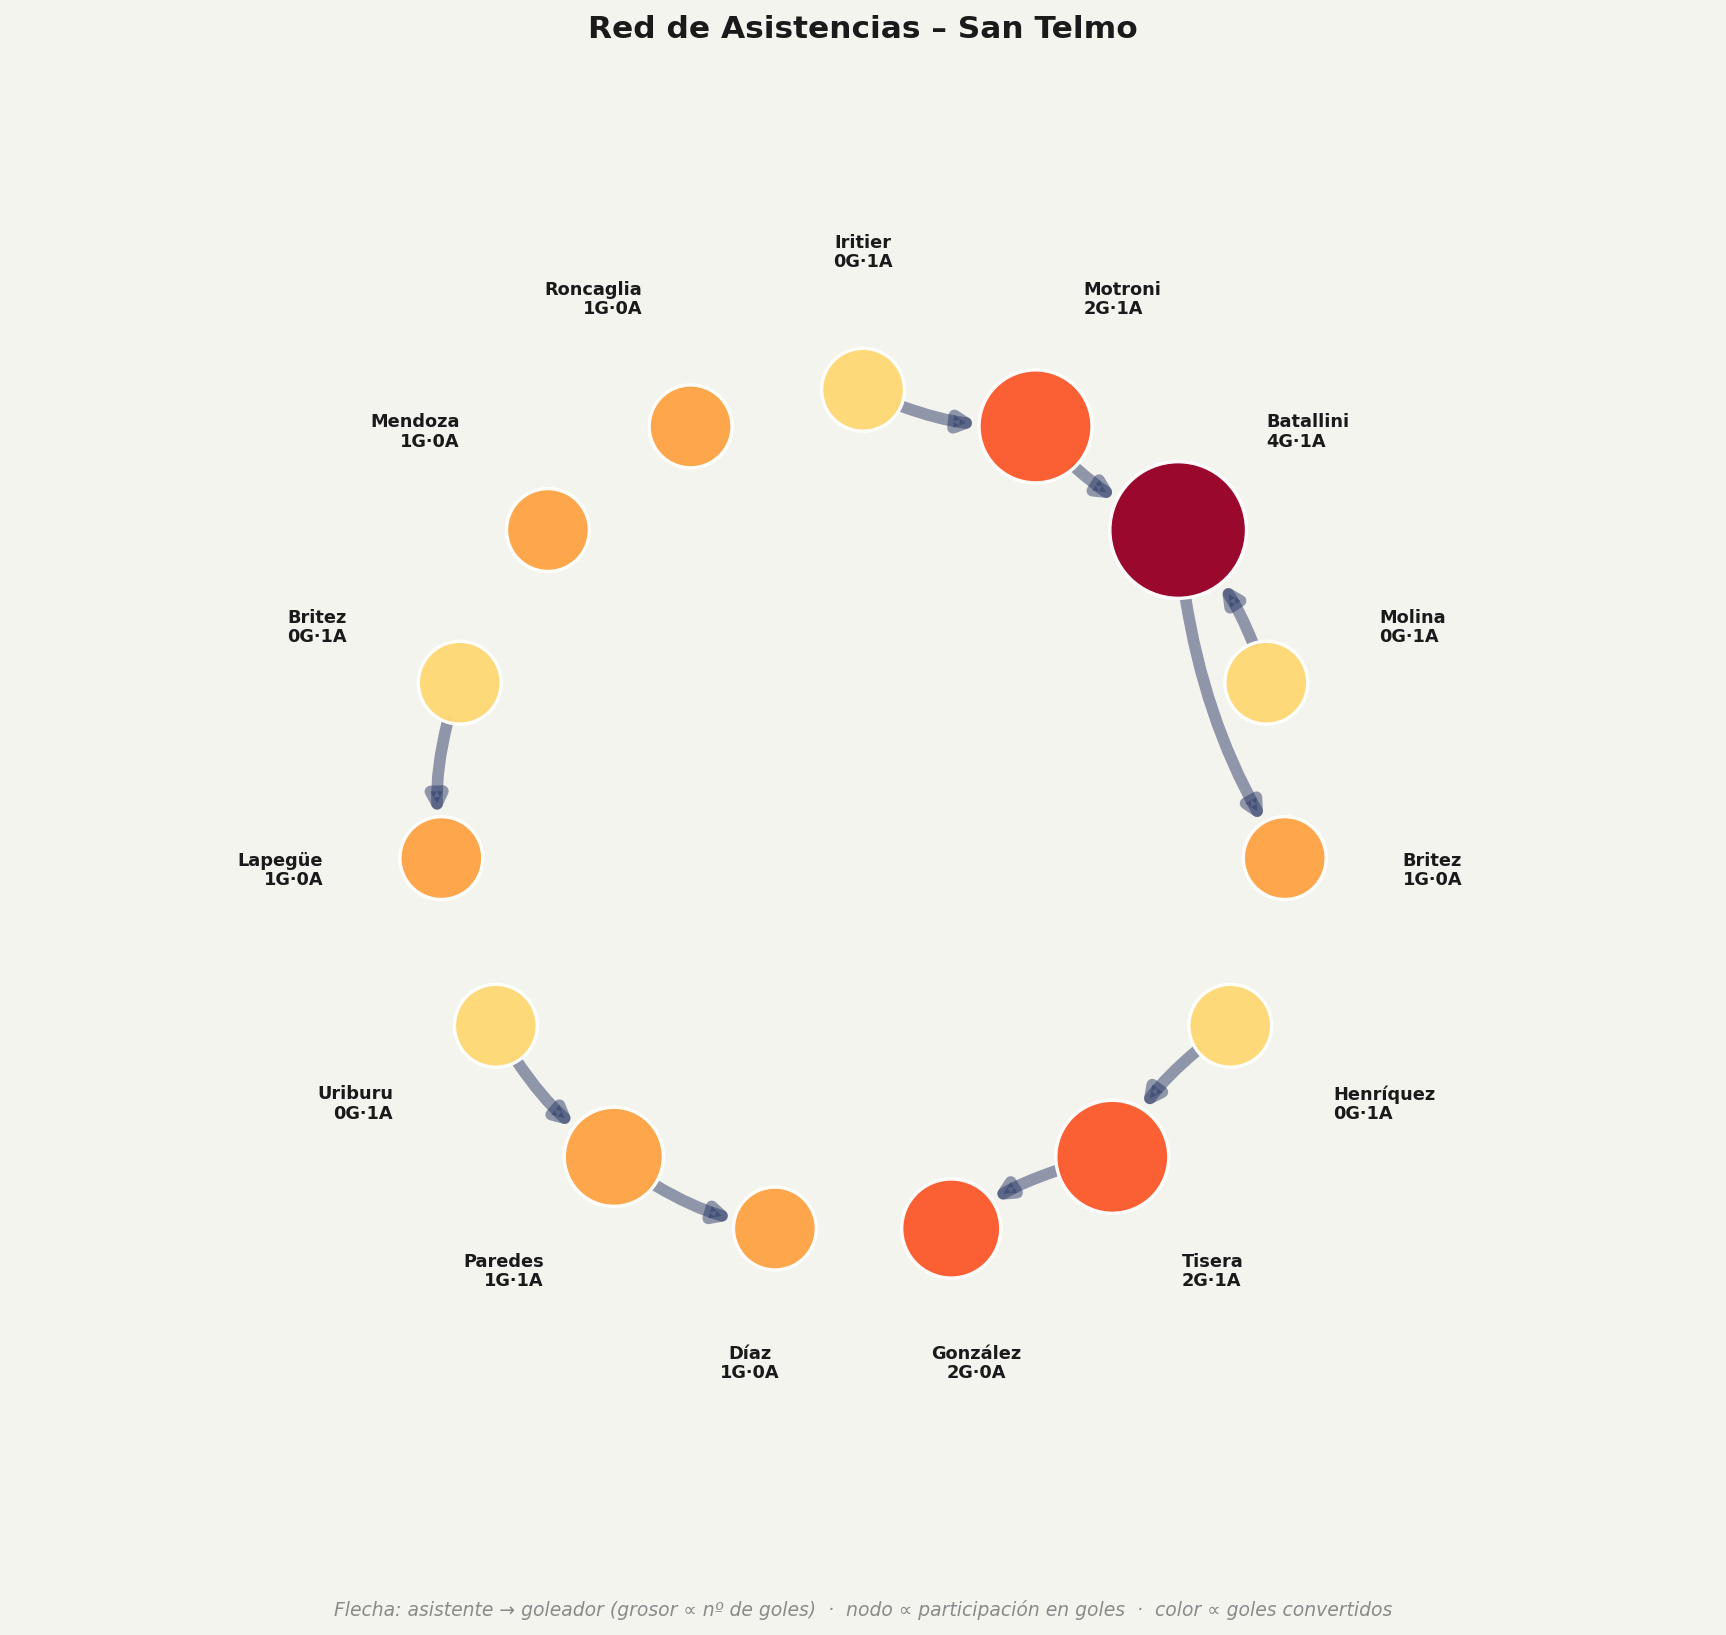
\includegraphics[width=0.9\textwidth]{red_asistencias.png}}
  \caption{Red de asistencias: quién habilita a quién en los goles.}
\end{figure}

\begin{figure}[htbp]
  \centering
  \fbox{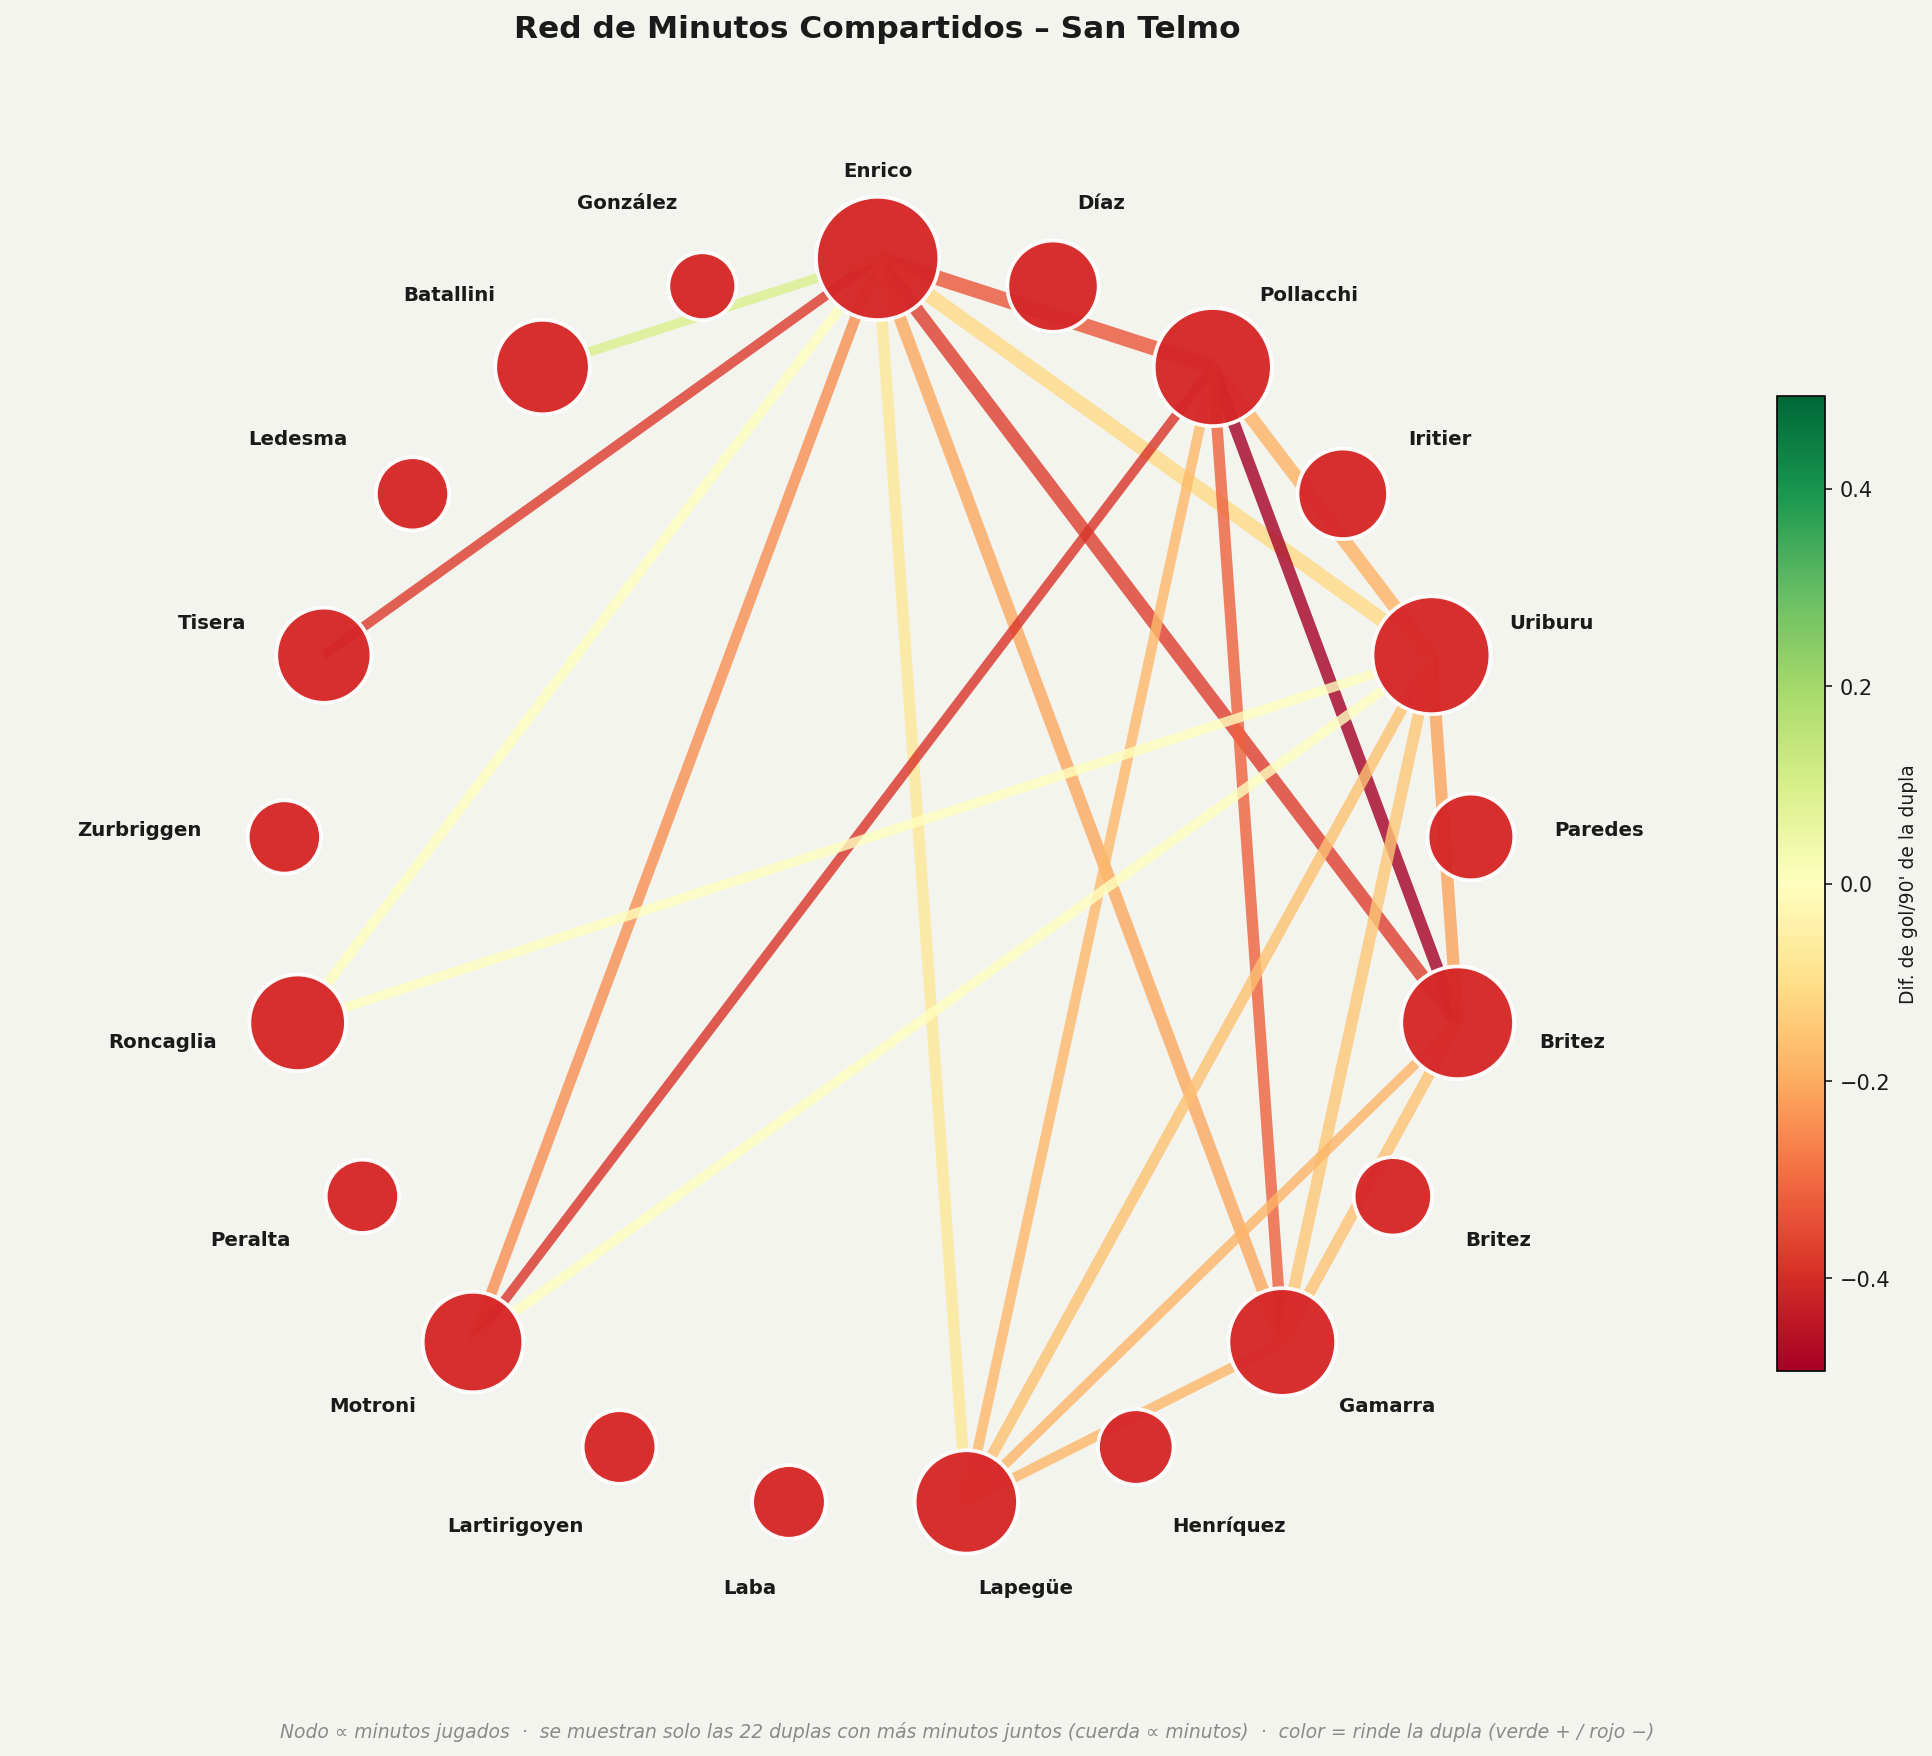
\includegraphics[width=0.9\textwidth]{red_minutos_compartidos.png}}
  \caption{Red de minutos compartidos: duplas más frecuentes y rendimiento del equipo con ellas.}
\end{figure}

\begin{figure}[htbp]
  \centering
  \fbox{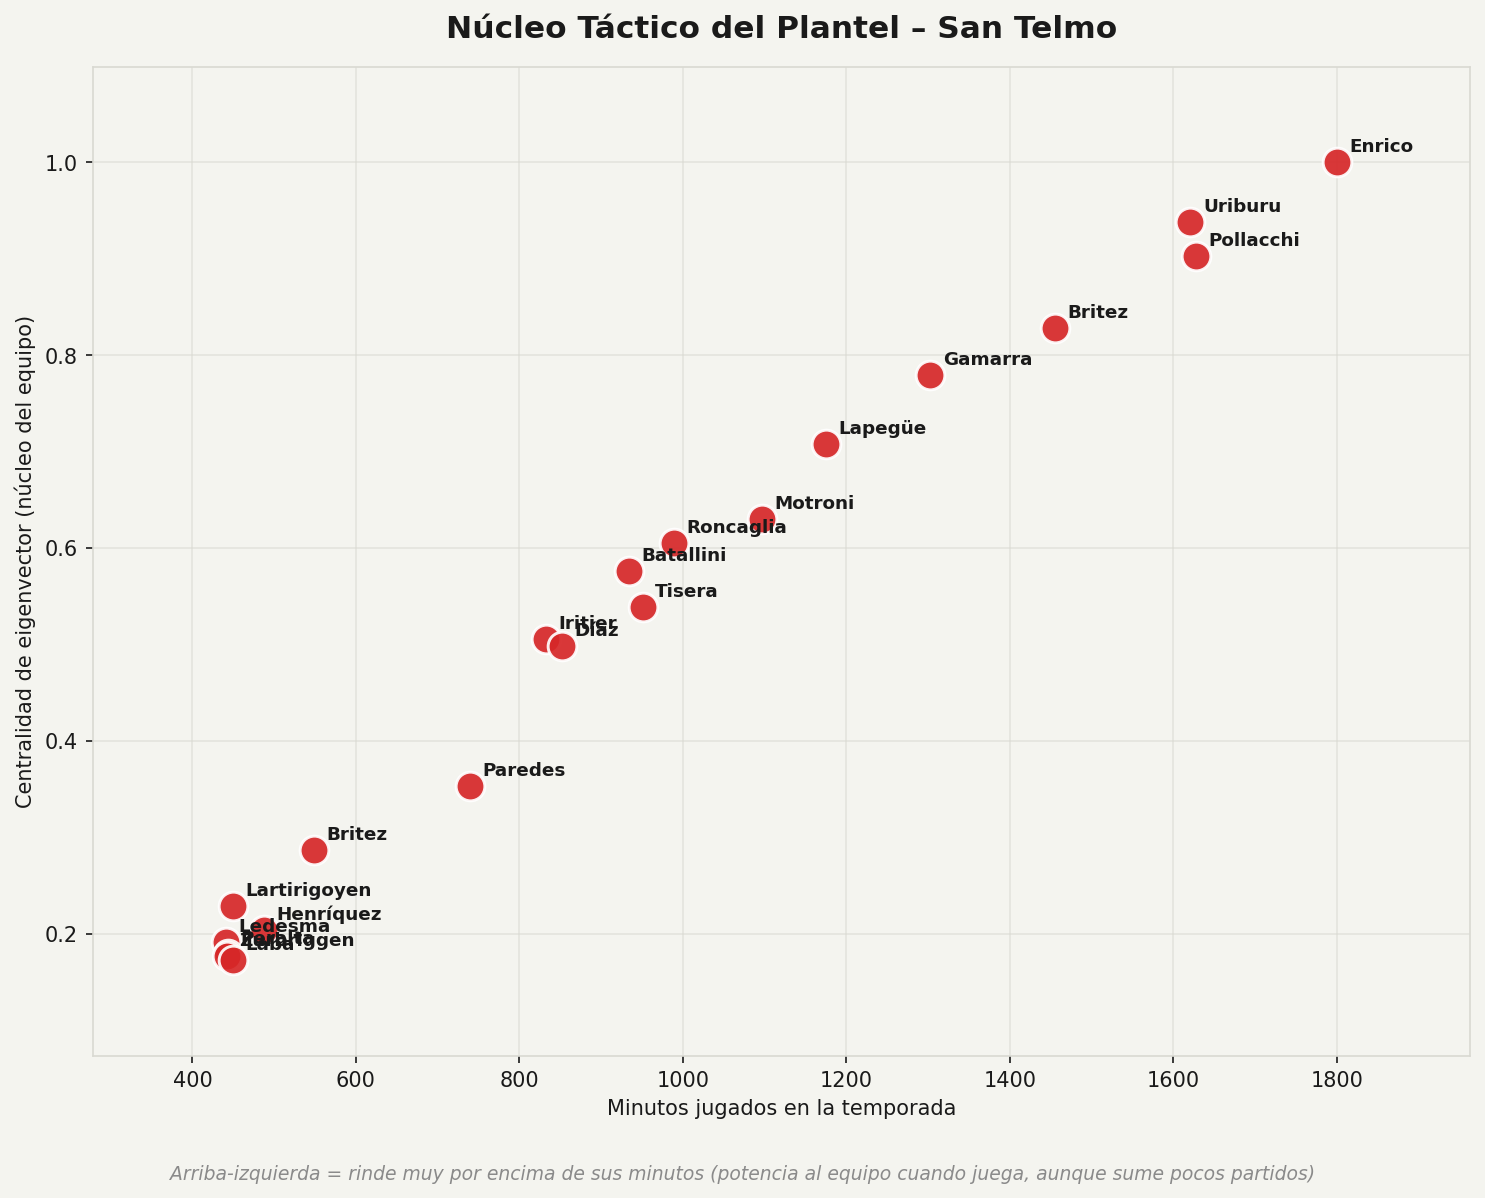
\includegraphics[width=0.85\textwidth]{nucleo_tactico.png}}
  \caption{Núcleo táctico (centralidad): jugadores que más potencian al equipo, más allá de sus números individuales.}
\end{figure}

\begin{figure}[htbp]
  \centering
  \fbox{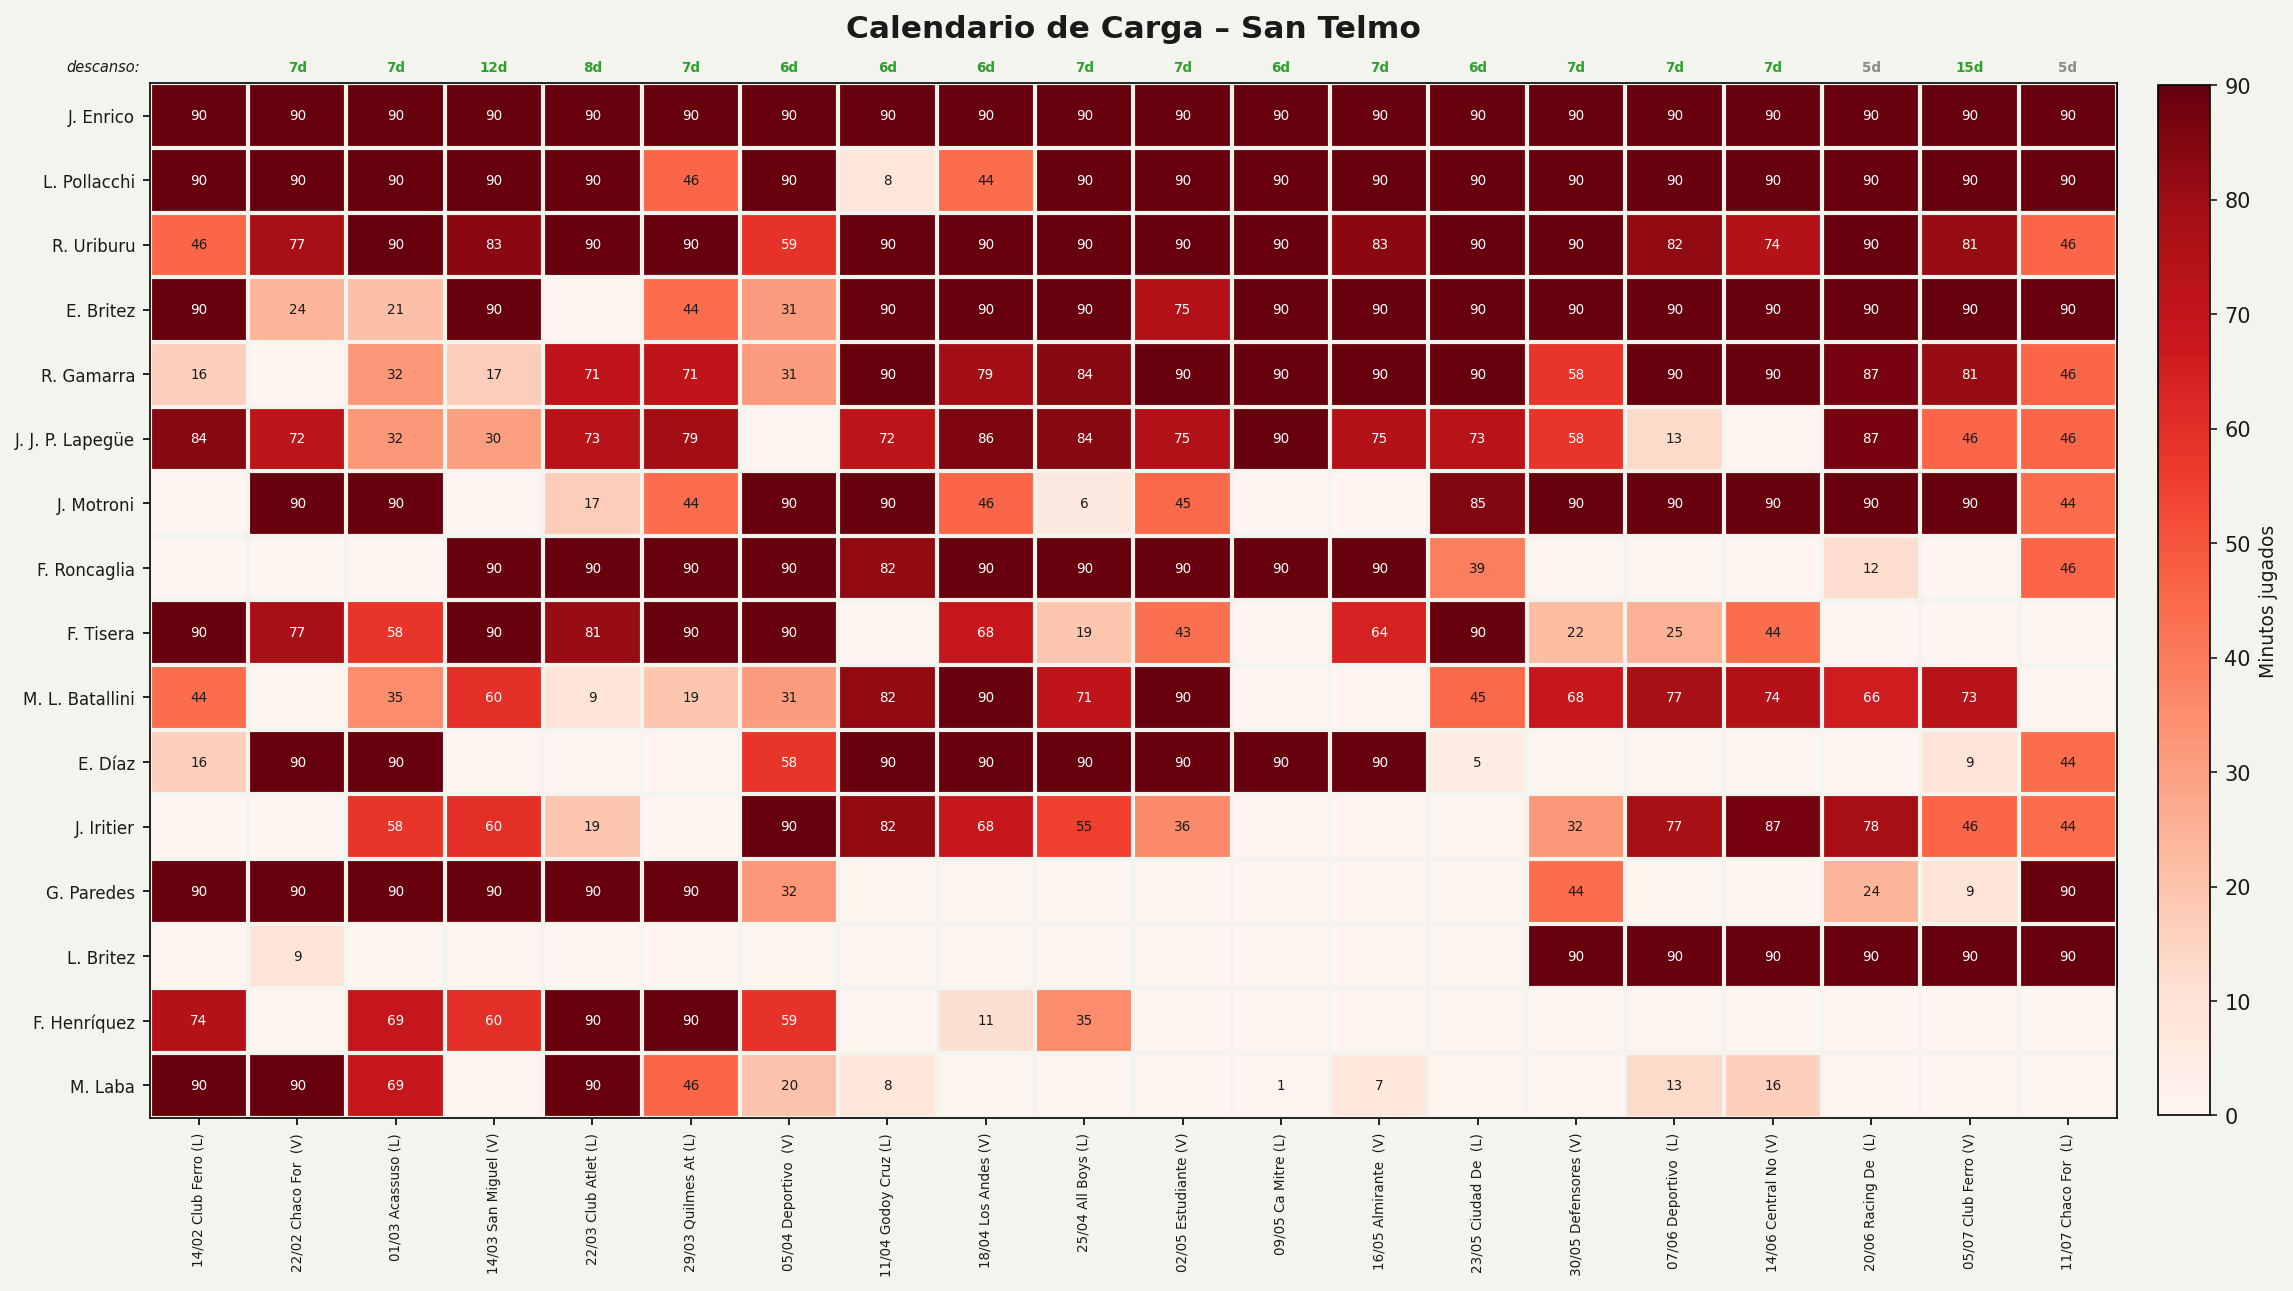
\includegraphics[width=0.98\textwidth]{calendario_carga.png}}
  \caption{Calendario de carga: minutos por jugador y descanso entre fechas (para decidir rotaciones).}
\end{figure}

\slot{jugadores clave, dependencias y decisiones de plantel}

\section*{5. Local vs. Visitante}
\begin{figure}[htbp]
  \centering
  \fbox{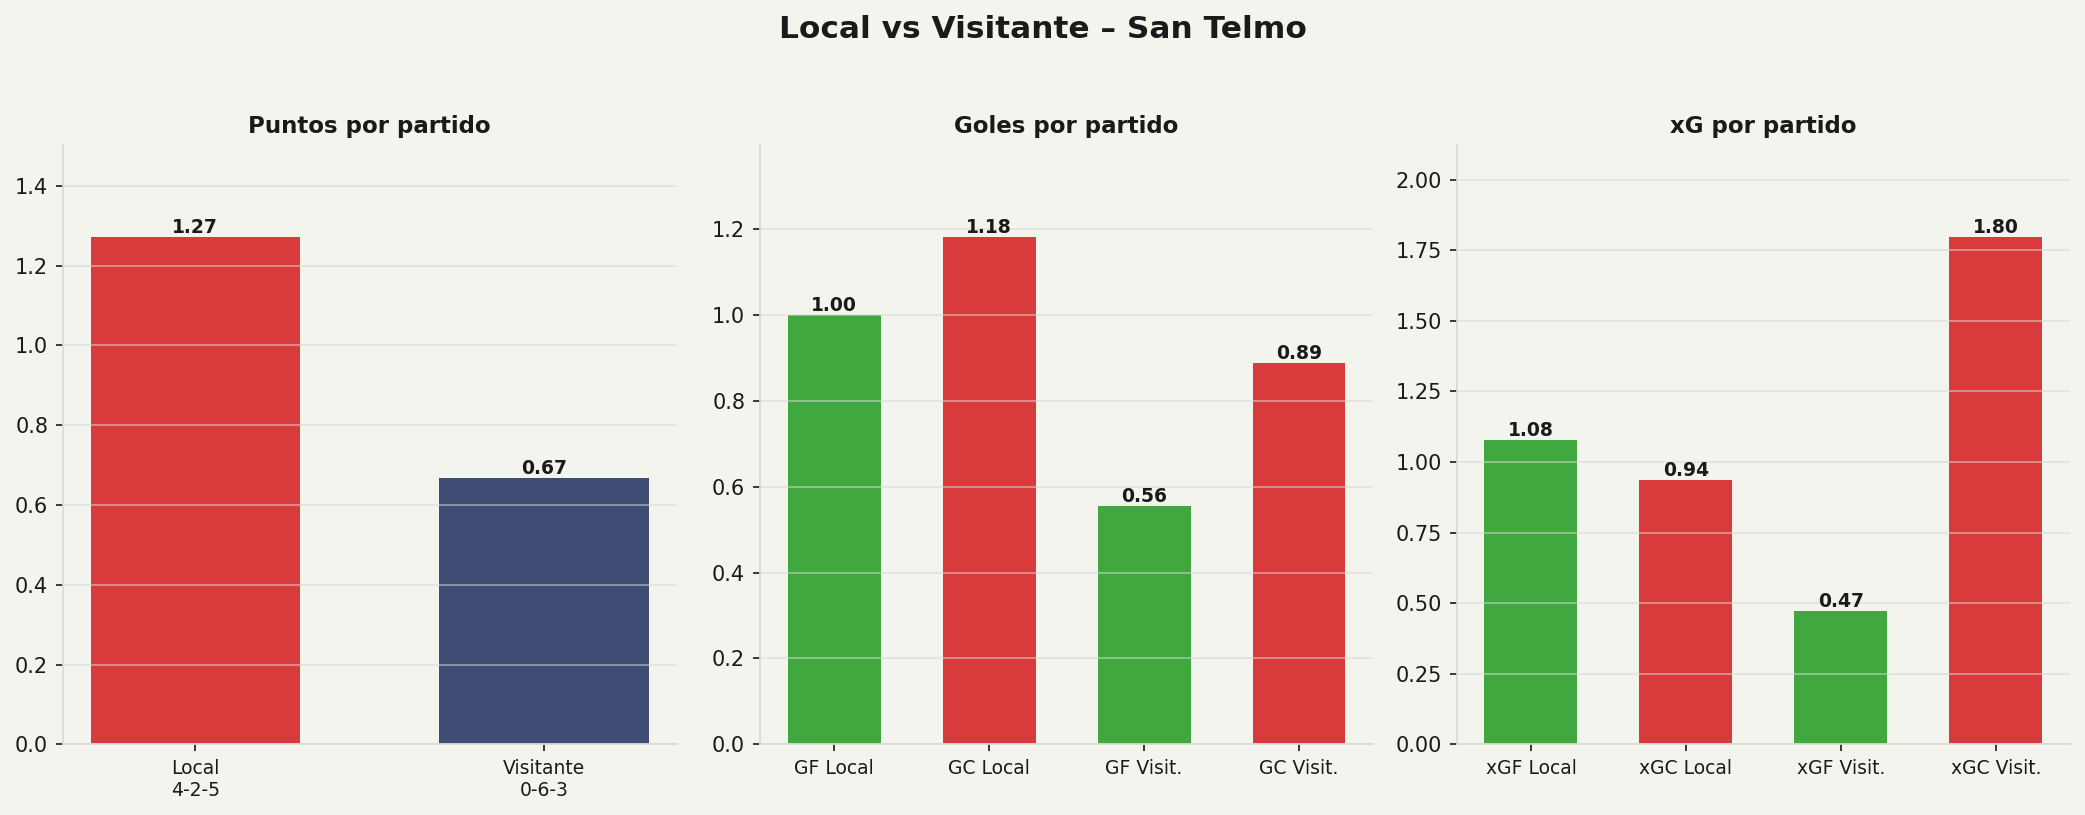
\includegraphics[width=0.85\textwidth]{local_vs_visitante.png}}
  \caption{Rendimiento según la condición: puntos, goles y xG por partido de local y de visitante.}
\end{figure}

\slot{diferencias de rendimiento según la cancha}

\section*{6. Conclusiones e Interpretación}
Hasta acá, los datos. Este espacio es para nuestra lectura del equipo y las recomendaciones que surjan del análisis.

\slot{síntesis del rendimiento, fortalezas y áreas de mejora}

\slot{recomendaciones concretas para el cuerpo técnico}

\end{document}
